\documentclass{beamer}
\usepackage[utf8]{inputenc}
\usepackage[T1]{fontenc}
\usepackage{import}

\usetheme{default}
\usecolortheme{seahorse}
\usefonttheme{serif}

% AMS and mathtools
\usepackage{amsmath,amsthm,amssymb,marvosym,mathrsfs,amsfonts,amscd,mathtools}

% Hyperlinks and URLs
\usepackage{url}
\usepackage{hyperref}
\hypersetup{
    colorlinks,
    citecolor=BLACK,
    filecolor=BLACK,
    linkcolor=BLACK,
    urlcolor=BLACK
}

% Bold math
\usepackage{bm}

% Bra Ket (Dirac) Notation
\usepackage{braket}

% Slashed characters (e.g. in Dirac equation)
\usepackage{slashed}

% Clean SI Units
\usepackage{siunitx}

% Enumerate thingies
\usepackage{enumitem}

% Cancel things out in equations
\usepackage[makeroom]{cancel}

% Graphics and figures
\usepackage{graphicx}
\usepackage{wrapfig}
\usepackage{float}

% Caption figures and tables
\usepackage{caption}

% Generate symbols
\usepackage{textcomp} % Include this line to avoid output errors
\usepackage{gensymb}

% Make multiple rows in a table
\usepackage{multirow}

% Booktabs tables
\usepackage{booktabs}

% Useful frames
\usepackage{mdframed}

% Comment-out large sections
\usepackage{comment}

% No auto-indent
\setlength{\parindent}{0pt}

% Asymptote - 3D vector graphics
\usepackage{asymptote}

% Tikz Package Stuff
\usepackage{pgf,tikz,pgfplots}
\usepackage[RPvoltages]{circuitikz}
\usepackage{tikz-3dplot}
% Use various tikz libraries
\usetikzlibrary{decorations.pathmorphing, decorations.markings, decorations.pathreplacing, patterns} % Decorate paths!
\usetikzlibrary{calc}
\usetikzlibrary{scopes}
\usetikzlibrary{angles, quotes}
\usetikzlibrary{svg.path}
\usetikzlibrary{arrows, arrows.meta}
\usetikzlibrary{fadings}
% pgfplots package settings
\pgfplotsset{compat=1.15}
% \pgfplotsset{width=10cm,compat=1.9} % Taken from latest overleaf.


% Awesome circled numbers
\newcommand*\circled[4]{\tikz[baseline=(char.base)]{\node[shape=circle, fill=#2, draw=#3, text=#4, inner sep=2pt] (char) {#1};}}

% Control size of text
\usepackage{relsize}

% Extend conditional commands
\usepackage{xifthen}

% Scale math by size
\newcommand*{\Scale}[2][4]{\scalebox{#1}{\ensuremath{#2}}}

% Big integrals
\usepackage{bigints}

% Number equations within sections
\numberwithin{equation}{section}

% Generate blind text
\usepackage{blindtext}

% Useful symbols
\usepackage{marvosym}


%%%% BLACKBOARD BOLD %%%%
\newcommand{\bbN}{\mathbb{N}} % Natural numbers
\newcommand{\bbZ}{\mathbb{Z}} % Zahlen
\newcommand{\bbQ}{\mathbb{Q}} % Rational numbers
\newcommand{\bbR}{\mathbb{R}} % Real numbers
\newcommand{\bbC}{\mathbb{C}} % Complex numbers
\DeclareSymbolFont{bbold}{U}{bbold}{m}{n} % Identity matrix
\DeclareSymbolFontAlphabet{\mathbbold}{bbold} % Identity matrix
\newcommand{\identitymatrix}{\mathbbold{1}} % Identity matrix


%%%% CODE LISTING %%%%
\usepackage{listings}
\definecolor{greencomments}{HTML}{00BA00}
\definecolor{graynumbers}{HTML}{4F4F4F}
\definecolor{purplestrings}{HTML}{AD00AA}
\definecolor{backgroundcolor}{HTML}{E8E8E8}
\lstdefinestyle{nkostin}{
    backgroundcolor=\color{backgroundcolor},   
    commentstyle=\color{greencomments},
    keywordstyle=\color{blue},
    numberstyle=\tiny\color{graynumbers},
    stringstyle=\color{purplestrings},
    basicstyle=\footnotesize,
    breakatwhitespace=false,         
    breaklines=true,                 
    captionpos=b,                    
    keepspaces=true,                 
    numbers=left,                    
    numbersep=5pt,                  
    showspaces=false,                
    showstringspaces=false,
    showtabs=false,                  
    tabsize=2
}
\lstset{style=nkostin}

%%%% UNIT BASIS VECTORS %%%%
\newcommand{\ihat}{\bm{\hat{\imath}}} % Cartesian i hat (x-direction)
\newcommand{\jhat}{\bm{\hat{\jmath}}} % Cartesian j hat (y-direction)
\newcommand{\khat}{\bm{\hat{k}}} % Cartesian k hat (z-direction)
\newcommand{\rhat}{\bm{\hat{r}}} % Spherical r hat
\newcommand{\phihat}{\bm{\hat{\phi}}} % Spherical phi hat
\newcommand{\thetahat}{\bm{\hat{\theta}}} % Spherical theta hat
\newcommand{\nhat}{\bm{\hat{n}}} % Unit normal vector
\newcommand{\rhohat}{\bm{\hat{\rho}}} % Cylindrical rho hat
\newcommand{\zhat}{\bm{\hat{z}}} % Cylindrical z hat


%%%% COLORS: DEFINITIONS AND COMMANDS %%%%
% Miscellaneous
\definecolor{DARKBLUE}{HTML}{040080}
\definecolor{DARKBROWN}{HTML}{8B4513}
\definecolor{LIGHTBROWN}{HTML}{CD853F}
\definecolor{PINK}{HTML}{D147BD}
\definecolor{LIGHTPINK}{HTML}{DC75CD}
\definecolor{GREENSCREEN}{HTML}{00FF00}
\definecolor{ORANGE}{HTML}{FF862F}
\newcommand{\DARKBLUE}{\color{DARKBLUE}}
\newcommand{\DARKBROWN}{\color{DARKBROWN}}
\newcommand{\LIGHTBROWN}{\color{LIGHTBROWN}}
\newcommand{\PINK}{\color{PINK}}
\newcommand{\LIGHTPINK}{\color{LIGHTPINK}}
\newcommand{\GREENSCREEN}{\color{GREENSCREEN}}
\newcommand{\ORANGE}{\color{ORANGE}}
% Blue
\definecolor{BLUEE}{HTML}{1C758A}
\definecolor{BLUED}{HTML}{29ABCA}
\definecolor{BLUEC}{HTML}{58C4DD}
\definecolor{BLUEB}{HTML}{9CDCEB}
\definecolor{BLUEA}{HTML}{C7E9F1}
\definecolor{BLUE}{HTML}{0000FF}
\newcommand{\BLUEE}{\color{BLUEE}}
\newcommand{\BLUED}{\color{BLUED}}
\newcommand{\BLUEC}{\color{BLUEC}}
\newcommand{\BLUEB}{\color{BLUEB}}
\newcommand{\BLUEA}{\color{BLUEA}}
\newcommand{\BLUE}{\color{BLUE}}
% Teal
\definecolor{TEALE}{HTML}{49A88F}
\definecolor{TEALD}{HTML}{55C1A7}
\definecolor{TEALC}{HTML}{5CD0B3}
\definecolor{TEALB}{HTML}{76DDC0}
\definecolor{TEALA}{HTML}{ACEAD7}
\definecolor{TEAL}{HTML}{00FFFF}
\newcommand{\TEALE}{\color{TEALE}}
\newcommand{\TEALD}{\color{TEALD}}
\newcommand{\TEALC}{\color{TEALC}}
\newcommand{\TEALB}{\color{TEALB}}
\newcommand{\TEALA}{\color{TEALA}}
\newcommand{\TEAL}{\color{TEAL}}
% Green
\definecolor{GREENE}{HTML}{699C52}
\definecolor{GREEND}{HTML}{77B05D}
\definecolor{GREENC}{HTML}{83C167}
\definecolor{GREENB}{HTML}{A6CF8C}
\definecolor{GREENA}{HTML}{C9E2AE}
\definecolor{GREEN}{HTML}{00FF00}
\newcommand{\GREENE}{\color{GREENE}}
\newcommand{\GREEND}{\color{GREEND}}
\newcommand{\GREENC}{\color{GREENC}}
\newcommand{\GREENB}{\color{GREENB}}
\newcommand{\GREENA}{\color{GREENA}}
\newcommand{\GREEN}{\color{GREEN}}
% Yellow
\definecolor{YELLOWE}{HTML}{E8C11C}
\definecolor{YELLOWD}{HTML}{F4D345}
\definecolor{YELLOWC}{HTML}{FFFF00}
\definecolor{YELLOWB}{HTML}{FFEA94}
\definecolor{YELLOWA}{HTML}{FFF1B6}
\definecolor{YELLOW}{HTML}{FFFF00}
\newcommand{\YELLOWE}{\color{YELLOWE}}
\newcommand{\YELLOWD}{\color{YELLOWD}}
\newcommand{\YELLOWC}{\color{YELLOWC}}
\newcommand{\YELLOWB}{\color{YELLOWB}}
\newcommand{\YELLOWA}{\color{YELLOWA}}
\newcommand{\YELLOW}{\color{YELLOW}}
% Gold
\definecolor{GOLDE}{HTML}{C78D46}
\definecolor{GOLDD}{HTML}{E1A158}
\definecolor{GOLDC}{HTML}{F0AC5F}
\definecolor{GOLDB}{HTML}{F9B775}
\definecolor{GOLDA}{HTML}{F7C797}
\newcommand{\GOLDE}{\color{GOLDE}}
\newcommand{\GOLDD}{\color{GOLDD}}
\newcommand{\GOLDC}{\color{GOLDC}}
\newcommand{\GOLDB}{\color{GOLDB}}
\newcommand{\GOLDA}{\color{GOLDA}}
% Red
\definecolor{REDE}{HTML}{CF5044}
\definecolor{REDD}{HTML}{E65A4C}
\definecolor{REDC}{HTML}{FC6255}
\definecolor{REDB}{HTML}{FF8080}
\definecolor{REDA}{HTML}{F7A1A3}
\definecolor{RED}{HTML}{FF0000}
\newcommand{\REDE}{\color{REDE}}
\newcommand{\REDD}{\color{REDD}}
\newcommand{\REDC}{\color{REDC}}
\newcommand{\REDB}{\color{REDB}}
\newcommand{\REDA}{\color{REDA}}
\newcommand{\RED}{\color{RED}}
% Maroon
\definecolor{MAROONE}{HTML}{94424F}
\definecolor{MAROOND}{HTML}{A24D61}
\definecolor{MAROONC}{HTML}{C55F73}
\definecolor{MAROONB}{HTML}{EC92AB}
\definecolor{MAROONA}{HTML}{ECABC1}
\newcommand{\MAROONE}{\color{MAROONE}}
\newcommand{\MAROOND}{\color{MAROOND}}
\newcommand{\MAROONC}{\color{MAROONC}}
\newcommand{\MAROONB}{\color{MAROONB}}
\newcommand{\MAROONA}{\color{MAROONA}}
% Purple
\definecolor{PURPLEE}{HTML}{644172}
\definecolor{PURPLED}{HTML}{715582}
\definecolor{PURPLEC}{HTML}{9A72AC}
\definecolor{PURPLEB}{HTML}{B189C6}
\definecolor{PURPLEA}{HTML}{CAA3E8}
\definecolor{PURPLE}{HTML}{FF00FF}
\newcommand{\PURPLEE}{\color{PURPLEE}}
\newcommand{\PURPLED}{\color{PURPLED}}
\newcommand{\PURPLEC}{\color{PURPLEC}}
\newcommand{\PURPLEB}{\color{PURPLEB}}
\newcommand{\PURPLEA}{\color{PURPLEA}}
\newcommand{\PURPLE}{\color{PURPLE}}
% White and Black
\definecolor{WHITE}{HTML}{FFFFFF}
\newcommand{\WHITE}{\color{WHITE}}
\definecolor{BLACK}{HTML}{000000}
\newcommand{\BLACK}{\color{BLACK}}
% Different Grays
\definecolor{LIGHTGRAY}{HTML}{BBBBBB}
\definecolor{GRAY}{HTML}{888888}
\definecolor{DARKGRAY}{HTML}{444444}
\definecolor{DARKERGRAY}{HTML}{222222}
\definecolor{GRAYBROWN}{HTML}{736357}
\newcommand{\LIGHTGRAY}{\color{LIGHTGRAY}}
\newcommand{\GRAY}{\color{GRAY}}
\newcommand{\DARKGRAY}{\color{DARKGRAY}}
\newcommand{\DARKERGRAY}{\color{DARKERGRAY}}
\newcommand{\GRAYBROWN}{\color{GRAYBROWN}}

\newcommand{\cat}[1][]{\tikz \fill [scale=1ex/500,yscale=1,#1] svg "M6125 12741 c-387 -139 -597 -254 -908 -495 -233 -181 -331 -236 -422 -236 -17 0 -69 11 -115 24 -115 33 -387 82 -540 97 -236 22 -573 0 -849 -56 -161 -33 -227 -39 -285 -25 -32 7 -108 48 -220 117 -381 238 -783 418 -1165 522 l-74 20 7 -87 c47 -605 193 -1137 396 -1443 l40 -60 -25 -65 c-38 -101 -93 -307 -116 -439 -18 -97 -22 -161 -23 -330 0 -213 11 -317 49 -441 26 -86 51 -79 -277 -76 -331 4 -697 -10 -1025 -38 -215 -19 -564 -59 -572 -66 -2 -2 -1 -9 2 -17 4 -11 27 -10 138 4 476 63 1214 101 1600 84 l167 -7 36 -87 c20 -47 55 -121 80 -163 l43 -77 -36 -5 c-20 -3 -92 -13 -161 -21 -513 -65 -1082 -183 -1506 -315 -194 -59 -234 -76 -234 -95 0 -8 1 -15 3 -15 2 0 57 18 122 40 266 90 566 168 900 234 276 55 413 76 891 141 l41 6 58 -77 c31 -42 88 -109 126 -149 l69 -72 -118 -43 c-265 -97 -648 -277 -882 -415 -179 -105 -370 -235 -370 -251 0 -8 4 -14 9 -14 4 0 69 40 142 89 339 225 742 426 1156 577 l93 33 93 -94 c214 -215 287 -380 287 -652 0 -260 -53 -544 -204 -1093 -70 -254 -124 -480 -156 -652 -157 -835 -108 -1553 159 -2358 89 -266 155 -431 312 -782 274 -611 310 -727 354 -1146 22 -205 36 -683 33 -1072 l-3 -345 -88 -7 c-109 -8 -232 -32 -290 -57 -66 -28 -111 -73 -143 -143 -26 -56 -29 -74 -29 -158 0 -74 4 -103 19 -129 67 -123 257 -196 611 -235 1310 -143 2603 -163 3865 -61 684 56 1558 169 1680 218 349 141 670 737 925 1721 185 712 354 1713 371 2201 24 650 -166 1275 -569 1880 -207 310 -356 484 -807 940 -477 483 -631 662 -805 935 -143 224 -273 537 -311 747 -35 198 -28 460 18 673 47 221 145 445 262 601 203 269 554 486 916 565 66 15 125 19 260 18 157 0 185 -3 274 -27 228 -61 359 -160 386 -292 26 -124 -55 -283 -190 -373 -135 -91 -278 -109 -464 -59 -131 35 -183 41 -236 27 -75 -19 -115 -52 -150 -124 -30 -61 -32 -71 -28 -144 6-97 36 -158 119 -238 71 -67 209 -135 321 -158 99 -20 253 -20 358 0 267 50 581 244 737 454 209 281 260 673 133 1013 -70 186 -311 431 -525 533 -206 98 -593 140 -925 99 -549 -68 -1041 -298 -1400 -654 -243 -242 -405 -492 -496 -769 l-37 -113 -56 6 c-135 13 -486 25 -753 25 -271 0 -289 1 -284 18 44 150 60 274 60 457 0 244 -33 410 -129 650 l-44 109 49 66 c252 342 406 715 456 1103 22 176 12 628 -15 627 -3 -1 -78 -27 -166 -59z m709 -3021 c88 -6 161 -11 162 -13 1 -1 -6 -42 -17 -92 -25 -119 -49 -305 -49 -377 0 -32 -3 -58 -6 -58 -3 0 -63 13 -132 29 -251 58 -593 119 -872 156 -69 9 -135 18 -147 21 -21 4 -20 8 32 117 29 61 61 138 71 169 18 53 21 57 54 62 57 7 732 -3 904 -14z m-604 -436 c173 -28 390 -71 666 -131 20 -5 21 -13 28 -166 27 -621 177 -1043 583 -1650 253 -378 580 -768 1023 -1222 273 -279 343 -357 438 -484 238 -315 387 -652 453 -1019 72 -406 36 -1045 -97 -1712 -160 -804 -476 -1596 -709 -1772 -91 -69 -196 -83 -285 -38 -126 65 -154 220 -111 605 12 105 37 318 56 475 62 523 75 690 75 955 0 641 -136 1169 -474 1844 -344 687 -592 1023 -1179 1597 -293 287 -426 407 -721 653 -143 120 -297 251 -340 292 -240 224 -359 512 -373 899 -4 114 -2 159 11 210 21 86 73 186 148 288 54 75 64 83 87 79 46 -10 341 -136 516 -222 207 -101 374 -196 564 -322 107 -71 146 -92 154 -84 8 8 8 14 2 19 -364 252 -809 488 -1172 621 -40 15 -60 27 -56 35 4 6 41 61 84 121 42 61 88 131 103 156 l26 46 143 -19 c78 -10 239 -34 357 -54Z";}

\newcommand{\iclicker}[1][]{\tikz \fill [scale=1ex/500,yscale=1,#1] svg "M2926 4713 c-20 -5 -20 -20 5 -194 l11 -75 111 4 c264 10 544 -47 751 -153 412 -210 616 -611 616 -1211 0 -145 -17 -130 158 -138 l112 -6 0 161 c0 181 -11 307 -41 459 -130 657 -600 1068 -1314 1150 -89 10 -373 12 -409 3z M2974 4173 c-10 -7 -1 -113 21 -238 l5 -30 123 -1 c356 -4 606 -166 708 -461 27 -79 49 -229 49 -340 l0 -93 43 0 c24 0 86 -3 137 -7 l93 -6 -6 169 c-11 315 -86 524 -251 701 -139 149 -307 240 -536 289 -82 17 -368 30 -386 17z M2400 4014 c-39 -14 -179 -150 -993 -963 -706 -704 -955 -959 -975 -996 -22 -41 -27 -63 -27 -125 0 -135 -23 -108 692 -821 710 -708 669 -674 808 -674 56 1 80 6 120 27 37 20 288 265 996 975 866 867 948 952 963 997 22 69 20 160 -5 216 -15 35 -169 195 -662 688 -386 387 -658 652 -682 664 -53 28 -172 34 -235 12z m413 -2396 l-918 -918 -612 612 -613 613 917 917 918 918 612 -612 613 -613 -917 -917z M2422 3271 c-126 -31 -216 -83 -313 -180 -69 -69 -94 -103 -128 -171 -93 -190 -95 -411 -6 -599 240 -505 967 -509 1216 -6 93 189 92 404 -3 605 -33 69 -57 100 -127 171 -71 70 -102 94 -171 127 -151 72 -315 90 -468 53z m240 -262 c123 -26 234 -115 289 -232 73 -158 37 -331 -97 -457 -243 -227 -636 -75 -670 259 -20 189 113 375 306 427 58 16 106 17 172 3z M2520 2742 c-55 -27 -83 -77 -78 -140 12 -145 203 -182 271 -52 22 43 18 111 -10 149 -24 33 -79 61 -118 61 -16 0 -46 -8 -65 -18z M1596 2170 c-100 -30 -135 -165 -64 -246 56 -63 149 -69 213 -13 65 57 71 149 14 214 -42 47 -100 63 -163 45z M1260 1851 c-104 -54 -109 -206 -10 -265 44 -25 124 -25 159 1 98 73 94 208 -9 261 -54 27 -94 28 -140 3z M1979 1737 c-124 -82 -67 -277 80 -277 153 0 209 200 79 280 -46 28 -115 26 -159 -3z M1680 1432 c-104 -52 -109 -212 -7 -267 51 -27 138 -17 177 20 80 77 58 209 -40 249 -52 21 -87 20 -130 -2z";}

\newcommand{\okay}[1][]{\tikz \fill [scale=1ex/500,yscale=1,#1] svg "M6608 12240 c-59 -10 -91 -36 -201 -163 -82 -94 -195 -264 -245 -367 -35 -73 -39 -77 -133 -138 -426 -279 -1060 -953 -1445 -1537 -171 -259 -221 -373 -421 -955 l-98 -285 -6 180 c-6 200 -23 277 -77 351 l-29 40 34 44 c82 106 143 256 184 446 29 137 38 428 15 533 -45 213 -170 338 -349 348 -47 3 -89 -1 -121 -11 -46 -14 -50 -14 -76 6 -38 28 -108 35 -148 14 -55 -28 -72 -83 -97 -308 -14 -124 -19 -143 -50 -195 -53 -90 -92 -201 -175 -500 -66 -236 -101 -421 -120 -628 -33 -367 -60 -480 -161 -690 -50 -103 -53 -115 -53 -185 0 -83 0 -83 132 -365 63 -136 96 -212 154 -360 65 -161 174 -484 224 -660 56 -198 64 -248 64 -400 0 -136 -4 -169 -40 -345 -22 -107 -60 -294 -85 -415 -131 -655 -391 -1910 -431 -2083 -93 -409 -209 -718 -401 -1070 -40 -73 -93 -165 -118 -203 -25 -39 -40 -67 -33 -63 7 4 4 -2 -7 -13 -12 -11 -50 -62 -85 -113 -127 -181 -292 -376 -507 -600 -45 -47 -80 -86 -78 -89 6 -6 142 103 214 171 182 174 331 344 470 537 64 90 101 146 198 306 44 71 126 228 177 335 163 348 248 640 361 1240 25 135 59 313 75 395 116 593 243 1352 270 1615 7 63 21 139 31 168 45 127 50 399 9 562 -33 132 -40 151 -53 143 -9 -5 -9 -3 -1 8 9 11 3 44 -27 149 -68 237 -173 535 -255 725 l-34 80 20 80 c11 44 32 97 46 118 22 33 23 38 8 35 -10 -2 -31 -25 -48 -51 -23 -38 -29 -59 -30 -107 0 -32 -1 -58 -2 -57 -1 1 -27 58 -58 126 l-56 125 24 31 c13 17 50 49 81 70 31 22 53 41 48 42 -18 6 -84 -28 -123 -63 l-40 -36 0 40 c0 28 16 71 54 148 94 189 115 282 151 656 13 142 31 299 40 350 18 105 32 124 119 157 28 10 44 21 38 25 -13 8 -91 -11 -110 -26 -7 -6 -14 -9 -17 -7 -8 9 125 506 155 579 39 94 78 157 156 246 111 129 154 208 154 283 l0 40 55 6 c102 13 203 -17 275 -82 100 -90 131 -197 130 -453 0 -306 -45 -510 -160 -727 -53 -102 -56 -108 -40 -98 11 7 32 -34 51 -100 10 -37 14 -111 13 -275 0 -349 -38 -547 -198 -1045 -47 -148 -76 -280 -86 -403 -6 -68 -8 -131 -5 -141 3 -10 6 -49 6 -87 1 -38 4 -87 8 -109 7 -36 8 -37 14 -15 3 14 8 99 11 190 3 111 11 196 25 260 21 95 176 577 192 595 5 5 9 16 9 26 0 20 141 438 240 714 40 110 92 255 116 322 70 197 68 193 106 193 43 0 192 36 226 55 l27 14 -25 1 c-14 0 -74 -11 -134 -25 -60 -14 -112 -23 -114 -20 -2 2 6 28 18 58 l22 54 62 12 c72 14 198 63 204 79 4 13 -113 -18 -198 -52 l-58 -24 17 42 c53 122 234 398 430 656 259 341 639 762 717 795 67 28 183 64 230 71 25 3 41 10 38 16 -9 14 -96 3 -175 -22 -35 -10 -64 -18 -66 -16 -5 5 221 203 315 274 186 141 290 196 527 274 83 27 171 61 198 76 70 38 132 109 151 173 19 64 19 92 1 144 -8 21 -13 40 -12 42 2 1 32 -17 68 -41 84 -57 154 -133 187 -204 24 -51 27 -68 27 -162 -1 -91 -5 -117 -32 -195 -47 -137 -149 -319 -269 -482 -64 -87 -311 -389 -361 -440 -42 -45 -53 -42 -53 13 0 57 -32 125 -78 165 -47 42 -66 36 -24 -8 53 -57 72 -106 72 -193 l0 -75 -92 -49 c-143 -76 -297 -169 -366 -221 -146 -110 -243 -232 -452 -570 -51 -82 -177 -285 -280 -450 -103 -165 -242 -390 -310 -500 -67 -110 -153 -249 -191 -308 -38 -59 -69 -110 -69 -113 0 -3 -13 -24 -29 -47 -16 -23 -60 -91 -97 -152 -37 -60 -97 -159 -134 -220 -159 -261 -344 -641 -380 -780 -11 -44 -23 -123 -25 -175 l-4 -95 14 70 c36 179 51 224 146 415 53 107 117 230 143 273 25 43 46 81 46 83 0 4 76 126 130 210 40 62 216 337 253 394 22 36 77 121 122 190 45 69 110 170 145 225 34 55 87 136 116 180 48 73 205 320 482 757 l106 167 20 -21 c11 -11 51 -35 90 -53 91 -42 116 -49 116 -35 0 6 -47 33 -105 60 -58 27 -105 55 -105 61 0 25 111 170 195 254 129 131 211 182 690 430 83 42 294 154 470 248 176 94 331 176 345 184 14 7 23 15 22 19 -2 3 0 9 4 12 4 4 4 1 -1 -7 -4 -7 -4 -12 1 -10 5 2 74 37 154 76 247 123 398 163 612 163 157 0 245 -10 468 -52 213 -41 363 -45 426 -11 23 12 60 43 82 68 l41 47 14 -34 c68 -163 27 -397 -103 -583 -98 -140 -303 -272 -550 -353 -90 -30 -352 -102 -370 -102 -4 0 3 26 16 58 28 69 38 130 30 177 -8 39 -26 48 -26 12 0 -84 -59 -188 -202 -352 -174 -201 -255 -268 -484 -408 -128 -77 -328 -210 -332 -219 -2 -4 -7 -8 -12 -8 -5 0 -46 -23 -92 -51 -46 -27 -115 -66 -155 -84 -72 -35 -97 -55 -69 -55 20 0 20 -8 -4 -115 -50 -225 -100 -354 -359 -915 l-81 -175 -232 -134 c-128 -73 -352 -201 -498 -283 -269 -152 -295 -168 -271 -168 37 0 569 266 941 470 681 374 982 531 1081 566 61 21 87 25 149 22 l75 -4 755 -378 c415 -208 770 -389 790 -401 63 -40 65 -46 53 -143 -6 -48 -10 -89 -8 -90 8 -9 36 62 42 104 l6 47 20 -39 c11 -21 38 -81 59 -133 38 -94 138 -290 196 -386 48 -79 132 -254 159 -329 34 -95 40 -178 18 -251 -19 -68 -69 -150 -112 -186 -39 -33 -133 -44 -358 -43 -135 0 -171 3 -231 22 -144 44 -263 152 -448 402 l-107 145 28 6 c15 4 46 7 69 8 169 5 411 137 496 270 42 67 34 70 -29 9 -108 -101 -215 -159 -364 -195 -99 -24 -310 -24 -433 1 -82 16 -296 74 -305 81 -2 2 26 61 61 132 56 112 103 237 122 326 11 50 -11 28 -39 -40 -163 -389 -390 -656 -751 -879 -155 -96 -223 -126 -276 -122 -42 3 -43 4 -50 45 -6 39 -33 103 -43 103 -2 0 -4 -40 -4 -88 1 -106 -11 -156 -58 -242 -62 -114 -235 -314 -264 -305 -17 6 -18 -1 -18 -69 0 -61 -7 -96 -41 -197 -56 -169 -82 -194 -150 -144 -60 44 -240 102 -240 77 0 -6 37 -30 82 -54 98 -52 179 -123 208 -183 12 -25 29 -84 39 -132 9 -47 22 -88 28 -90 6 -2 13 18 17 48 8 60 0 62 137 -23 185 -115 334 -279 631 -699 75 -107 159 -221 185 -254 87 -108 158 -140 250 -115 62 17 173 127 258 255 98 147 174 245 265 339 140 146 217 201 430 309 84 42 90 47 55 42 -22 -2 -67 -13 -100 -24 -33 -11 -61 -18 -64 -15 -13 13 -11 216 3 284 29 144 207 448 364 627 171 193 367 298 598 319 57 5 77 3 105 -11 19 -10 30 -19 24 -21 -5 -1 -22 -5 -37 -8 -40 -9 -89 -55 -111 -106 -18 -39 -21 -71 -25 -230 -4 -162 -2 -196 17 -273 33 -138 74 -207 137 -227 40 -13 96 7 114 40 6 12 14 20 16 17 2 -2 9 -42 15 -88 23 -193 60 -332 153 -577 72 -191 72 -269 -2 -421 -41 -85 -90 -152 -352 -482 -102 -128 -196 -248 -210 -266 -14 -17 -99 -125 -190 -239 -190 -239 -280 -353 -463 -589 -232 -297 -350 -405 -631 -574 -155 -93 -432 -241 -574 -308 -51 -23 -90 -47 -87 -53 3 -5 0 -7 -8 -4 -7 2 -69 -20 -138 -51 -378 -171 -643 -281 -1444 -598 -302 -119 -459 -187 -451 -194 6 -6 36 4 249 78 92 33 171 59 175 59 3 0 -31 -25 -77 -55 -240 -160 -421 -340 -578 -575 -91 -136 -158 -293 -148 -347 2 -10 4 -26 4 -35 2 -30 18 -20 25 15 36 190 444 660 806 928 74 55 151 112 170 128 19 15 53 34 75 41 261 83 1006 380 1390 553 145 66 535 266 650 334 305 182 427 290 666 593 249 314 629 809 629 819 0 6 4 11 9 11 8 0 390 489 488 625 134 186 176 356 128 517 -8 29 -40 115 -71 191 -64 159 -117 359 -140 532 -12 92 -15 187 -12 405 l3 285 -27 46 c-34 58 -77 87 -189 128 l-26 10 49 52 c28 29 64 80 81 114 29 56 31 67 32 165 0 85 -5 118 -24 175 -29 85 -56 137 -65 128 -4 -4 -4 0 -1 8 3 9 -45 115 -115 252 -67 131 -135 274 -151 318 -64 176 -110 241 -217 313 -63 41 -673 355 -1267 652 -316 158 -343 165 -472 140 -124 -24 -306 -115 -828 -416 -55 -32 -115 -65 -134 -75 l-34 -17 22 33 c12 19 55 93 96 166 196 343 286 612 289 859 l1 101 75 23 c41 13 107 40 145 60 94 49 185 99 215 118 14 9 98 58 188 109 195 111 283 175 377 274 85 89 126 140 194 239 l51 74 178 36 c211 43 295 68 422 123 237 102 383 232 475 422 58 119 75 191 75 313 0 160 -41 258 -163 391 -119 130 -175 132 -497 24 -74 -26 -200 -73 -280 -106 -137 -56 -151 -60 -260 -67 -273 -20 -405 -69 -925 -345 -44 -23 -152 -80 -240 -125 -88 -46 -218 -114 -288 -152 -71 -37 -131 -68 -134 -68 -4 0 68 75 158 168 243 247 366 409 460 607 138 288 126 514 -36 677 -25 26 -72 63 -103 82 -64 39 -178 80 -193 70 -6 -3 -25 4 -41 16 -38 28 -82 38 -130 30z m140 -52 c46 -22 72 -73 72 -140 0 -70 -23 -121 -75 -166 -56 -50 -108 -71 -315 -127 -36 -10 -106 -36 -157 -57 -51 -21 -95 -38 -98 -38 -20 0 340 473 390 512 13 10 34 22 47 28 27 12 100 5 136 -12z m2277 -707 c22 -10 45 -24 52 -33 13 -15 34 -190 22 -182 -4 2 -14 -7 -22 -20 -9 -13 -36 -33 -60 -45 -63 -30 -149 -27 -356 14 -97 19 -227 41 -290 49 -62 8 -115 16 -116 18 -2 2 92 33 208 69 117 37 244 79 282 93 152 59 215 67 280 37z m-5396 -772 c22 -8 30 -16 27 -28 -3 -9 -8 -29 -12 -46 -11 -45 -64 -121 -144 -205 -70 -73 -72 -74 -65 -40 4 19 18 88 30 155 22 123 37 161 65 169 30 8 67 6 99 -5z m4488 -3789 c67 -22 161 -46 210 -54 50 -7 94 -16 100 -19 6 -4 34 -48 63 -99 128 -226 256 -381 369 -448 91 -53 166 -73 283 -74 54 -1 98 -2 98 -2 0 -1 -24 -14 -52 -29 -171 -89 -329 -252 -457 -468 -85 -146 -141 -265 -162 -345 -25 -100 -25 -237 1 -312 10 -30 18 -55 17 -56 -1 -1 -33 -17 -72 -37 -81 -40 -161 -97 -260 -185 -92 -83 -164 -166 -300 -347 -154 -207 -198 -244 -270 -231 -43 8 -85 55 -273 304 -223 295 -266 347 -391 473 -149 149 -293 245 -418 278 -44 12 -45 13 -57 91 -4 20 -17 55 -30 80 l-23 44 31 15 c35 18 84 94 117 181 22 57 30 172 17 222 -7 24 -3 29 40 54 26 15 86 66 133 113 103 104 157 201 166 300 5 52 9 61 22 56 68 -26 140 -8 301 77 226 119 412 270 536 435 l54 72 43 -24 c23 -13 97 -42 164 -65z m1655 -743 c57 -53 69 -126 48 -307 -6 -52 -11 -157 -12 -233 0 -135 -1 -138 -29 -177 -71 -98 -145 -39 -185 149 -20 92 -29 381 -15 455 12 66 27 87 90 127 47 31 56 29 103 -14z";}

\newcommand{\bunny}[1][]{\tikz \fill [scale=1ex/500,yscale=1,#1] svg "M3831 8683 c-70 -71 -235 -358 -326 -567 -168 -385 -252 -748 -275 -1181 -5 -104 -9 -199 -7 -209 2 -16 -10 -21 -88 -36 -158 -31 -407 -112 -530 -173 -117 -58 -239 -150 -365 -277 -178 -177 -305 -366 -407 -604 -44 -102 -55 -118 -136 -201 -110 -113 -148 -183 -154 -288 -4 -53 0 -88 14 -132 12 -37 16 -70 12 -85 -4 -14 -7 -62 -8 -107 -3 -225 125 -386 369 -461 66 -20 157 -35 282 -47 l68 -7 -25 -47 c-41 -81 -59 -197 -52 -341 10 -200 66 -413 174 -660 153 -347 352 -632 640 -914 l104 -102 9 -95 c13 -131 12 -378 -1 -441 -25 -115 -92 -205 -180 -242 -138 -58 -168 -77 -220 -139 -92 -109 -110 -180 -63 -237 63 -75 165 -100 429 -107 159 -4 215 -2 275 11 267 57 455 273 539 619 20 84 29 107 41 103 8 -3 89 -37 179 -76 197 -86 466 -177 651 -220 74 -18 142 -34 150 -37 8 -3 -14 -15 -50 -28 -257 -88 -340 -205 -227 -319 48 -47 82 -58 257 -78 225 -26 1652 -9 1850 23 75 12 154 51 184 92 22 30 23 43 15 268 -3 65 0 83 25 133 50 102 131 161 255 187 46 9 67 8 150 -11 230 -54 428 -7 556 131 71 77 99 149 92 240 -7 115 -65 203 -185 282 -218 145 -282 308 -264 665 30 563 -100 1035 -383 1397 -78 99 -236 254 -335 327 -319 238 -731 392 -1245 468 -301 44 -438 49 -1090 37 -69 -2 -107 3 -160 20 l-70 22 3 238 c3 183 0 265 -12 356 -18 123 -53 275 -81 340 -16 38 -16 40 9 70 456 567 686 1088 725 1647 21 289 -41 691 -116 749 -28 23 -72 27 -106 10 -63 -31 -322 -342 -452 -541 -38 -59 -73 -108 -77 -108 -5 0 -8 11 -8 24 0 14 -9 74 -21 133 -44 228 -158 517 -217 547 -50 26 -80 20 -121 -21z";} 


\title{PHGN 200 --- Electromagnetism and Optics}
\subtitle{Block II: Circuits}

\author{}
\date{Block II Review Slides}

\begin{document}

\frame{\titlepage}

\begin{frame}{A Quick Introduction}

\begin{center}
Block I was all about \emph{electrostatics} --- we dealt with stationary charges.
\end{center}

\vfill

\begin{center}
Now we're in Block II, and we care about what happens when charges are mobilized in circuits.
\end{center}

\vfill

\begin{center}
So let's start at the beginning and consider \emph{moving} charges.
\end{center}

\end{frame}

\begin{frame}{Current}

Current is moving charge. Nothing more, nothing less. Mathematically, current is given by
\begin{equation*}
    I = \frac{dQ}{dt}
\end{equation*}

We can think of current as the \emph{charge per unit time} passing a given point. Current is measured in coulombs-per-second, or \textbf{amperes} (A):
\begin{equation*}
    \SI{1}{\ampere} = \SI{1}{\coulomb/\second}
\end{equation*}

\end{frame}

\begin{frame}{A Historical Confusion --- Blame Ben Franklin}

In practice, it is ordinarily the negatively charged electrons that do the moving --- in the direction \emph{opposite} to the electric current.

\begin{figure}[H]
\centering
\begin{circuitikz}
    \draw (0,0) to[battery,i>=$I$] (0,3);
    \draw (0,3) to (1.5,3) node[label={[font=\tiny]above:$\textcolor{BLUE}{\longleftarrow \text{electron flow} \longleftarrow}$}] {} to (3,3);
    \draw (3,3) to[resistor,i>=$I$] (3,0);
    \draw (3,0) to (0,0);
    \draw (3,0) to (1.5,0) node[label={[font=\tiny]below:$\textcolor{BLUE}{\longrightarrow \text{electron flow} \longrightarrow}$}] {} to (0,0);
\end{circuitikz}
\end{figure}

To avoid complicating things, we often pretend it's the positive charges that move. That is, we don't care about the direction the electrons move (and instead only focus on the flow of positive charges).

\end{frame}

\begin{frame}{Worked Example --- Finding how much Charge Passed a Given Point}

$\blacktriangleright$ Suppose the current at some point in a wire is given by the function $I(t) = I_o e^{-t/2}$, where $I_o = \SI{2.2}{\ampere}$.

\begin{figure}[H]
\centering
\begin{tikzpicture}[scale=0.6]
\begin{axis}[axis lines = center, xlabel = $t$, ylabel = {$I(t)$}]
% \addplot[domain=0:10, samples=200, color=blue] {-0.4*sin(1.7453*deg(x))+2};
\addplot[domain=0:16, samples=200, color=blue] {2.2*exp(-x/2)};
\end{axis}
\end{tikzpicture}
\end{figure}

How much charge passes through that point in the wire?

\end{frame}

\begin{frame}{Worked Example --- Finding how much Charge Passed a Given Point}

\textit{Solution.} Current is defined by $I = \frac{dQ}{dt}$. This implies that a differential amount of charge is given by
\begin{equation*}
    dQ = I\ dt
\end{equation*}

Then we can find the \emph{total} amount of charge by integrating:
\begin{equation*}
    Q = \int dQ = \int I\ dt
\end{equation*}
    
\end{frame}

\begin{frame}{Worked Example --- Finding how much Charge Passed a Given Point}

So we know that integrating $I$ with respect to time gives us charge. But what time do we integrate over?

\vfill

We're looking for the \emph{total charge} that goes through that point in the circuit. So we might as well integrate over all time.

\vfill

\textit{Pause and Ponder:} Where would we see a physical example of such a current?

\end{frame}

\begin{frame}{Worked Example --- Finding how much Charge Passed a Given Point}

Integrating, we get
\begin{align*}
    Q = \int dQ &= \int I\ dt \\
                &= \int_{0}^{\infty} \left( I_o e^{-t/2} \right)\ dt \\
                &= I_o \left( -2 e^{-t/2} \right) \bigg|_{0}^{\infty} \\
                &= \left( \SI{2}{\second} \right) I_o
\end{align*}

Thus, the total charge that passes through that point in the circuit is
\begin{equation*}
    \left( \SI{2}{\second} \right) \left( \SI{2.2}{\ampere} \right) = \boxed{ \SI{4.4}{\coulomb} = Q } \blacktriangleleft
\end{equation*}

\end{frame}

\begin{frame}{Another Definition of Current}

Consider a some conductor where the density of charge-carriers is $n$ (and each has charge $q$), the cross-sectional area is $A$, and the drift velocity of the charge carriers is $v_d$. Then the current is
\begin{equation*}
    I = n \left|q\right| v_d A
\end{equation*}

If the charge carriers are electrons, then their charge is $e_f = \SI{1.602e-19}{\coulomb}$, and the current is
\begin{equation*}
    I = n e_f v_d A
\end{equation*}

Additionally, we can consider just the \emph{current per unit area} which is known as the current density:
\begin{equation*}
    J = \frac{I}{A} = n q v_d
\end{equation*}

\begin{center}
(Current density will come back in Block III.)
\end{center}

\end{frame}

\begin{frame}{Voltage}

So we've established what \emph{current} is. It's nothing more than \emph{moving charges}. But how did we get these charges moving in the first place? They certaintly don't move on their own, right?

\vfill

Voltage is defined to be the amount of \emph{energy per unit charge}. The change in energy by some charge $q$ in moving from point $a$ to point $b$ is

\begin{equation*}
    \Delta U = q \left( V_b - V_a \right) = q \Delta V
\end{equation*}

\vfill

(The energy that actually drives charges can come from a battery --- in which case a chemical reaction is supplying the energy.)

\end{frame}

\begin{frame}{Resistance}

Resistance is a way of quantifying how much effort it takes to move charge across less-than-perfect conductors. Experimentally, we find that, for most materials

\begin{equation*}
    R = \frac{\varrho\ L}{A} \quad \implies \quad dR = \frac{\varrho\ dL}{A}
\end{equation*}

where $\varrho$ is the electrical resistivity, measured in ohm-meter (\si{\ohm\cdot\metre}), $L$ is the length of the resistor, and $A$ is the cross-sectional area.
    
\end{frame}

\begin{frame}{Worked Example --- Resistance of a Goofy Resistor}

$\blacktriangleright$ Suppose a solid ``lampshade'' has height $h$ and base radii $a$ and $a/2$. Wires are attached to the ends of the ``lampshade'' as shown below:

\begin{figure}[H]
\centering
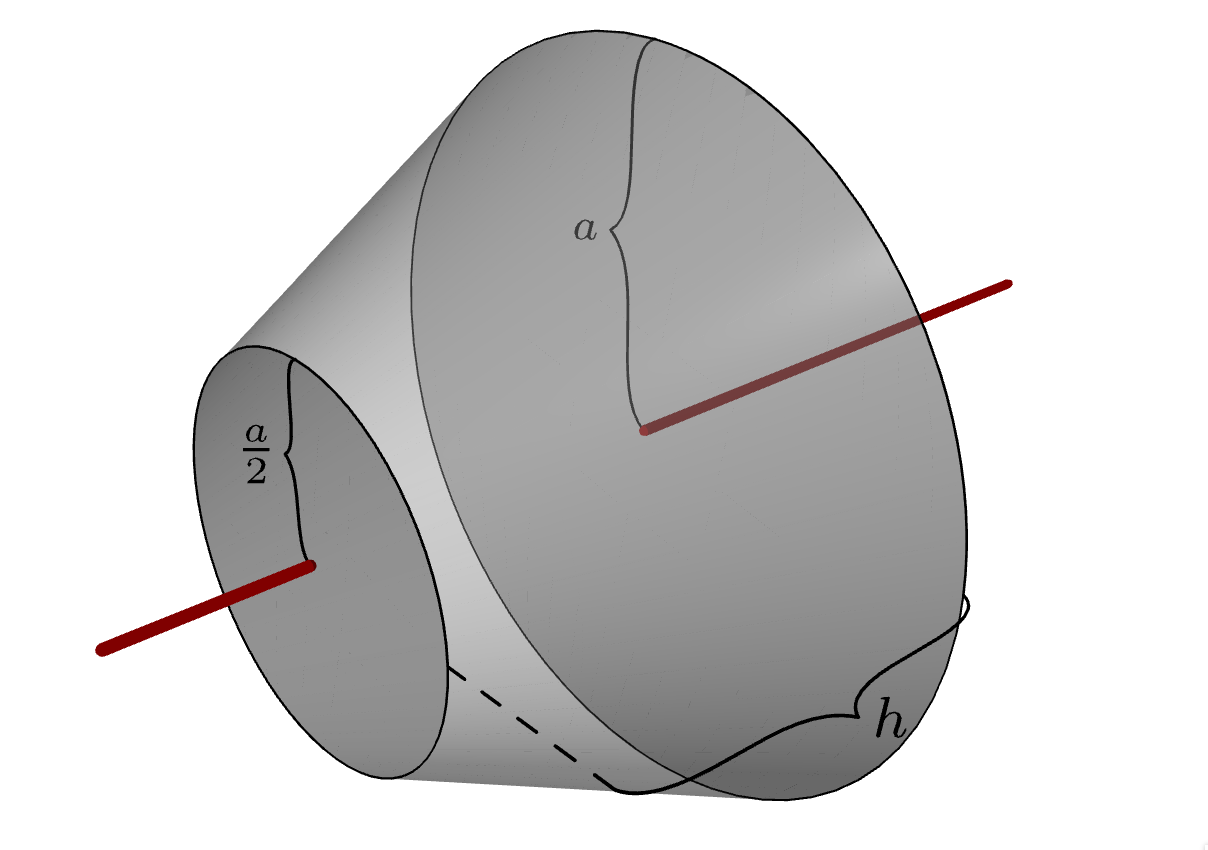
\includegraphics[height=0.5\textheight]{figures/half.png}
\end{figure}

Given that the cone has resistivity $\varrho$, what is the resistance of such a configuration?

\end{frame}

\begin{frame}{Worked Example --- Resistance of a Goofy Resistor}

\textit{Solution.} We want to find the resistance of some goofy ``lampshade'' resistor. As such, we'll want to start with the familiar expression for differential resistance:

\begin{equation*}
    dR = \frac{\varrho\ dL}{A}
\end{equation*}

This is our governing equation. Now let's build it up.

\end{frame}

\begin{frame}{Worked Example --- Resistance of a Goofy Resistor}

For the sake of simplicity, let's make the axis of the ``lampshade'' the $x$-axis, with the smaller base at $x = 0$.

\begin{figure}[H]
\centering
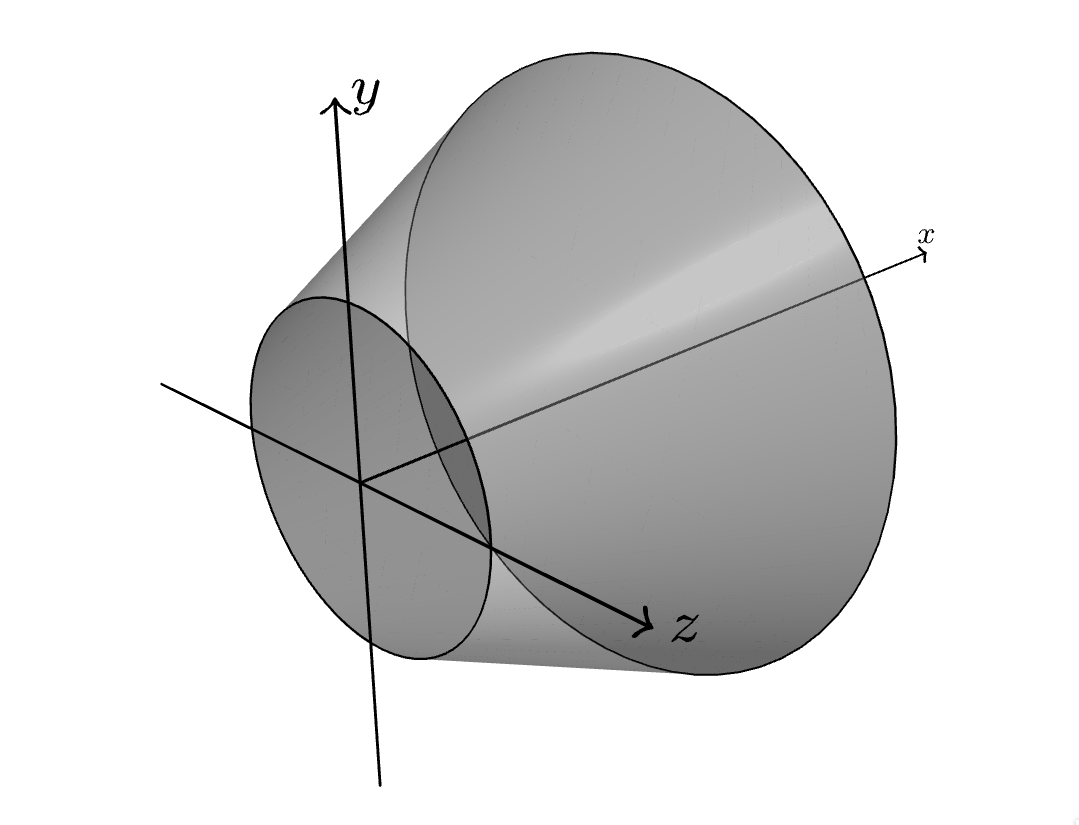
\includegraphics[height=0.5\textheight]{figures/lamponx.png}
\end{figure}

Then $dL$ --- the differential length through the resistor --- is $dx$.

\end{frame}

\begin{frame}{Worked Example --- Resistance of a Goofy Resistor}

What about the area? The area in the expression $dR = \frac{\varrho\ dL}{A}$ refers to the \emph{cross-sectional} area that the current ``sees'' when moving through the resistor. In our case: circles!

\begin{figure}[H]
\centering
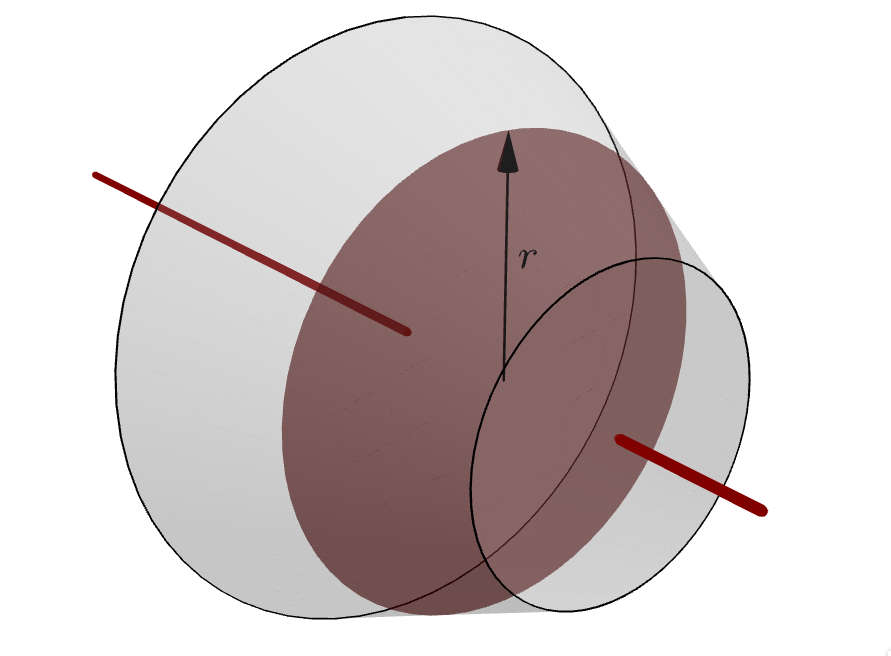
\includegraphics[height=0.5\textheight]{figures/lampcirc.png}
\end{figure}

And we know the area of a circle is $\pi r^2$. But what \emph{exactly} is the radius?

\end{frame}

\begin{frame}{Worked Example --- Resistance of a Goofy Resistor}

Let's look at the ``lampshade'' from the side.

\begin{figure}[H]
\centering
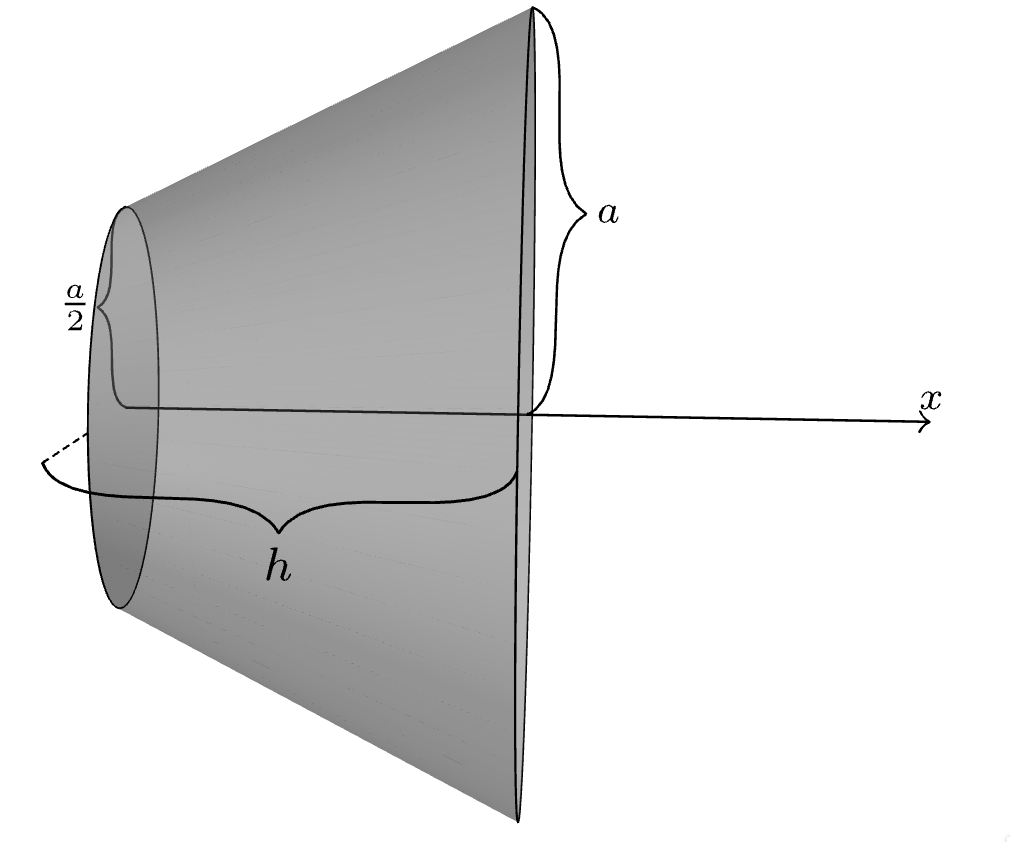
\includegraphics[height=0.3\textheight]{figures/whatradius.png}
\end{figure}

We can deduce that the radius $r$ as a function of the position $x$ along the $x$-axis is
\begin{equation*}
    r = \frac{a}{2h} x + \frac{a}{2} = \frac{a \left(x + h\right)}{2h}
\end{equation*}

And thus the \emph{cross-sectional} area as a function of the position $x$ along the $x$-axis is
\begin{equation*}
    A = \pi \left[ \frac{a \left(x + h\right)}{2h} \right]^2 = \frac{\pi a^2 \left(x + h\right)^2}{4h^2}
\end{equation*}

\end{frame}

\begin{frame}{Worked Example --- Resistance of a Goofy Resistor}

All that's left is to put everything together and integrate. We have
\begin{align*}
    R = \int dR &= \int_{0}^{h} \frac{(4h^2) \varrho\ dx}{\pi a^2\ \left( x + h \right)^2} \\
                &= \frac{(4h^2) \varrho}{\pi a^2} \int_{0}^{h} \frac{dx}{\left(x + h\right)^2} \\
                &= \frac{(4h^2) \varrho}{\pi a^2} \left( -\frac{1}{x + h} \right) \bigg|_{0}^{h}
\end{align*}

So in conclusion, the resistance of the entire configuration is
\begin{equation*}
    \boxed{R = \frac{2 h \varrho}{\pi a^2}} \blacktriangleleft
\end{equation*}

\end{frame}

\begin{frame}{Resistors in Series}

Resistors can be arranged in series:

\begin{figure}[H]
\centering
\begin{circuitikz}
    \draw (0,0) to[R,l^=$R_1$] (2,0);
    \draw (2,0) to[R,l^=$R_2$] (4,0);
    \draw (4,0) to[R] (6,0);
    \draw (6,0) to[R,l^=$R_n$] (8,0);
\end{circuitikz}
\end{figure}

\begin{center}
Resistors in series carry the same current.
\end{center}

\vfill

The equivalent resistance of $n$ resistors in series is
\begin{equation*}
    R_{\text{eq}} = R_1 + R_2 + \cdots + R_n
\end{equation*}

\end{frame}

\begin{frame}{Resistors in Parallel}

Resistors can also be arranged in parallel:

\begin{figure}[H]
\centering
\begin{circuitikz}
    \draw (0,0) to (6,0);
    \draw (0,0) to[R,l^=$R_1$] (0,2);
    \draw (2,0) to[R,l^=$R_2$] (2,2);
    \draw (4,0) to[R] (4,2);
    \draw (6,0) to[R,l^=$R_n$] (6,2);
    \draw (0,2) to (6,2);
\end{circuitikz}
\end{figure}

\begin{center}
Resistors in parallel are subject to the same voltage drop.
\end{center}

\vfill

The equivalent resistance of $n$ resistors in parallel is
\begin{gather*}
    \frac{1}{R_{\text{eq}}} = \frac{1}{R_1} + \frac{1}{R_2} + \cdots + \frac{1}{R_n} \\
    \implies R_{\text{eq}} = \left( \frac{1}{R_1} + \frac{1}{R_2} + \cdots + \frac{1}{R_n} \right)^{-1}
\end{gather*}

\end{frame}

\begin{frame}{Ohm's Law}

So we know that current $I$ is nothing more than moving charges. In a circuit, a difference in voltage $\Delta V$ (say, from a battery) drives the movement of these charges. And since these charges probably move across less-than-perfect conductors, they encounter a resistance $R$. 

\vfill

These quantities are related by \emph{Ohm's Law}, which reads
\begin{equation*}
    \Delta V = IR
\end{equation*}

In other words, the voltage difference $\Delta V$ across a load with resistance $R$ is proportional to the current $I$.

\end{frame}

\begin{frame}{Energy and Power in Circuits}

The power dissipated by a circuit component is
\begin{equation*}
    P = I \left( \Delta V \right)
\end{equation*}

For \emph{ohmic} material (that is, where Ohm's law applies), this becomes
\begin{equation*}
    P = I \left( \Delta V \right) = I^2 R = \frac{\left( \Delta V \right)^2}{R}
\end{equation*}

Now say I want to calculate the energy dissipated by some circuit component over a period of time from $t_i$ to $t_f$. Power is defined as the time derivative of energy so 
\begin{gather*}
    P \equiv \frac{dU}{dt} \quad \implies \quad dU = P\ dt \\
    \implies U = \int_{t_i}^{t_f} P\ dt
\end{gather*}

\end{frame}

\begin{frame}{Kirchhoff's Current Law}

The sum of the currents entering a junction is equal to the sum of the currents leaving a junction:

\begin{equation*}
    \underbrace{\hspace{2em}\sum I_{\text{in}} = \sum I_{\text{out}}\hspace{2em}}_{\parbox[c]{0.8\textwidth}{\begin{center} This is a statement of charge conservation \end{center}}}
\end{equation*}

\vfill

Note that a junction is any place on a circuit where three or more wires meet.

\end{frame}

\begin{frame}{Kirchhoff's Voltage Law}

The sum of voltage drops around a closed loop is zero:

\begin{equation*}
    \underbrace{\hspace{2em}\sum \Delta V = 0 \quad \text{for any closed loop}\hspace{2em}}_{\parbox[c]{0.8\textwidth}{\begin{center} This is a statement of energy conservation \end{center}}}
\end{equation*}

\end{frame}

\begin{frame}{How to Use Kirchhoff's Voltage Law}

For any closed loop in a circuit: 

\begin{enumerate}

\item[(1)] Choose a starting location and go all the way around the loop, returning to where you started. Go either \emph{clockwise} or \emph{counterclockwise} --- but be consistent!

\item[(2)] As you encounter a circuit element (whether that's a battery, emf source, capacitor, or a resistor) decide whether there's a \textcolor{GREENE}{positive} or \textcolor{RED}{negative} contribution to $\Delta V$ according to the following sign conventions:

\begin{itemize}

\item[$\bullet$] Crossing a battery (or emf source) from the \emph{negative} terminal to the \emph{positive} terminal gives a \textcolor{GREENE}{positive contribution to $\Delta V$}

\item[$\bullet$] Crossing a capacitor from the \emph{negative} plate to the \emph{positive} plate gives a \textcolor{GREENE}{positive contribution to $\Delta V$}

\item[$\bullet$] Crossing a resistor in the direction of \emph{positive current flow} gives a \textcolor{RED}{negative contribution to $\Delta V$}

\item[$\bullet$] Vice versa for all the above

\end{itemize}

\end{enumerate}

\end{frame}

\begin{frame}{Worked Example --- Kirchhoff Analysis}

$\blacktriangleright$ The following diagram shows a circuit where: $R_1 = \SI{8.0}{\ohm}$, $R_2 = \SI{7.0}{\ohm}$, $R_3 = \SI{4.0}{\ohm}$, $V_1 = \SI{4.2}{\volt}$, $V_2 = \SI{18.0}{\volt}$, and $V_3 = \SI{4.5}{\volt}$. What is the value of $I_1$?

\begin{figure}[H]
\centering
\begin{circuitikz}
    \draw (0,0) to[battery,l^=$V_1$] (0,1.3);
    \draw (0,0.9) to[resistor,l^=$R_1$,i>=$\textcolor{BLUE}{I_1}$] (0,3);
    \draw (0,3) to[battery,invert,l^=$V_2$] (0,4);
    \draw (0,0) to (3,0);
    \draw (0,4) to (3,4);
    \draw (3,0) to[resistor,l^=$R_2$,i>=$\textcolor{BLUE}{I_2}$] (3,4);
    \draw (3,0) to (6,0);
    \draw (3,4) to (6,4);
    \draw (6,0) to[battery,invert,l^=$V_3$,i>=$\textcolor{BLUE}{I_3}$] (6,2.4);
    \draw (6,2) to[resistor,l^=$R_3$] (6,4);
    % \draw (0,0) to[battery,i>=$I$] (0,3);
    % \draw (0,3) to (1.5,3) node[label={[font=\tiny]above:$\textcolor{BLUE}{\longleftarrow \text{electron flow} \longleftarrow}$}] {} to (3,3);
\end{circuitikz}
\end{figure}

\end{frame}

\begin{frame}{Worked Example --- Kirchhoff Analysis}

\textit{Solution.} Let's start with the junction equations. Kirchhoff's Junction Law reads

\begin{equation*}
    \sum I_{\text{in}} = \sum I_{\text{out}}
\end{equation*}

And there are two junctions on our circuit:

\begin{figure}[H]
\centering
\begin{circuitikz}[scale=1.0]
    \draw (0,0) to[battery,l^=$V_1$] (0,1.3);
    \draw (0,0.9) to[resistor,l^=$R_1$,i>=$\textcolor{BLUE}{I_1}$] (0,3);
    \draw (0,3) to[battery,invert,l^=$V_2$] (0,4);
    \draw (0,0) to (3,0);
    \draw (0,4) to (3,4);
    \draw (3,0) to[resistor,l^=$R_2$,i>=$\textcolor{BLUE}{I_2}$] (3,4);
    \draw (3,0) to (6,0);
    \draw (3,4) to (6,4);
    \draw (6,0) to[battery,invert,l^=$V_3$,i>=$\textcolor{BLUE}{I_3}$] (6,2.4);
    \draw (6,2) to[resistor,l^=$R_3$] (6,4);
    \draw (3,3) to[short,-*,color=red] (3,4) node[label={[font=\small]above:$\textcolor{RED}{\text{Top Junction}}$}] {} to (3,3);
    \draw (3,1) to[short,-*,color=red] (3,0) node[label={[font=\small]below:$\textcolor{RED}{\text{Bottom Junction}}$}] {} to (3,1);
\end{circuitikz}
\end{figure}

\end{frame}

\begin{frame}{Worked Example --- Kirchhoff Analysis}

For the top junction, we have:
\begin{equation*}
    \underbrace{\hspace{0.2em} I_1 + I_2 + I_3 \hspace{0.2em}}_{\parbox[c]{0.4\textwidth}{\begin{center} \vspace{-0.7em} \tiny All three currents entering junction \end{center}}} \hspace{-2em} = \hspace{-3em} \overbrace{\hspace{1.4em} 0 \hspace{1.4em}}^{\parbox[c]{0.4\textwidth}{\begin{center} \tiny No currents leaving \vspace{-1em} \end{center}}}
\end{equation*}

And for the bottom junction:
\begin{equation*}
    \underbrace{\hspace{1.4em} 0 \hspace{1.4em}}_{\parbox[c]{0.2\textwidth}{\begin{center} \vspace{-0.7em} \tiny No currents entering junction \end{center}}} \hspace{-1em} = \hspace{-2em} \overbrace{\hspace{0.2em} I_1 + I_2 + I_3 \hspace{0.2em}}^{\parbox[c]{0.4\textwidth}{\begin{center} \tiny All three currents leaving \vspace{-1em} \end{center}}}
\end{equation*}

These two equations are saying the same thing, and we don't need that redundancy. So the junction equation is:
\begin{equation*}
    I_1 + I_2 + I_3 = 0
\end{equation*}

\end{frame}

\begin{frame}{Worked Example --- Kirchhoff Analysis}

Now it's time to look at the loop equations. (Let's go clockwise)

\begin{figure}[H]
\centering
\begin{circuitikz}
    \draw (0,0) to[battery,l^=$V_1$] (0,1.3);
    \draw (0,0.9) to[resistor,l^=$R_1$,i>=$\textcolor{BLUE}{I_1}$] (0,3);
    \draw (0,3) to[battery,invert,l^=$V_2$] (0,4);
    \draw (0,0) to (3,0);
    \draw (0,4) to (3,4);
    \draw (3,0) to[resistor,l^=$R_2$,i>=$\textcolor{BLUE}{I_2}$] (3,4);
    \draw (3,0) to (6,0);
    \draw (3,4) to (6,4);
    \draw (6,0) to[battery,invert,l^=$V_3$,i>=$\textcolor{BLUE}{I_3}$] (6,2.4);
    \draw (6,2) to[resistor,l^=$R_3$] (6,4);
\end{circuitikz}
\end{figure}

For the loop on the left:

\begin{equation*}
    +V_1 - I_1 R_1 - V_2 + I_2 R_2 = 0
\end{equation*}

And for the loop on the right:

\begin{equation*}
    -I_2 R_2 + I_3 R_3 + V_3 = 0
\end{equation*}

\end{frame}

\begin{frame}{Worked Example --- Kirchhoff Analysis}

Let's take a look at what happens when we add the equations for the left and right loops:

\begin{align*}
    V_1 - I_1 R_1 - V_2 + \cancel{I_2 R_2} &= 0 \\
    (+) \qquad \cancel{-I_2 R_2} + I_3 R_3 + V_3 &= 0 \\
    \cline{1-2}
    V_1 - I_1 R_1 - V_2 + I_3 R_3 + V_3 &= 0
\end{align*}

\begin{center}
This is exactly the equation for the big loop (that encompasses the whole circuit)!
\end{center}

\vfill

This tells us that the big loop equation is redundant so we won't include it. (After all, we already have three equations for our three unknowns $I_1$, $I_2$, and $I_3$.)

\end{frame}

\begin{frame}{Worked Example --- Kirchhoff Analysis}

So to summarize what we have so far:
\begin{align*}
    \text{Left loop:}&& V_1 - I_1 R_1 - V_2 + I_2 R_2 &= 0 \\
    \text{Right loop:}&& -I_2 R_2 + I_3 R_3 + V_3 &= 0 \\
    \text{Junction:}&& I_1 + I_2 + I_3 &= 0
\end{align*}

\vfill

Now we just have to solve for $I_1$. To do so, let's solve for $I_2$ and $I_3$ in terms of $I_1$ and plug everything into the junction equation.

\end{frame}

\begin{frame}{Worked Example --- Kirchhoff Analysis}

Solving the left loop equation for $I_2$ gives
\begin{equation*}
    I_2 = \frac{I_1 R_1 + V_2 - V_1}{R_2}
\end{equation*}

And solving the right loop equation for $I_3$ gives
\begin{equation*}
    I_3 = \frac{I_2 R_2 - V_3}{R_3}
\end{equation*}

Into which we can sub in what we just found for $I_2$:
\begin{equation*}
    I_3 = \frac{\overbrace{\left( \frac{I_1 R_1 + V_2 - V_1}{R_2} \right)}^{I_2} R_2 - V_3}{R_3} = \frac{I_1 R_1 + V_2 - V_1 - V_3}{R_3}
\end{equation*}

Awesome. Now we have $I_2$ and $I_3$ in terms of $I_1$.

\end{frame}

\begin{frame}{Worked Example --- Kirchhoff Analysis}

Now let's plug everything into the junction equation:
\begin{equation*}
    I_1 + \overbrace{\left( \frac{I_1 R_1 + V_2 - V_1}{R_2} \right)}^{I_2} + \overbrace{\left( \frac{I_1 R_1 + V_2 - V_1 - V_3}{R_3} \right)}^{I_3} = 0
\end{equation*}

And, after a bit of tedious work, we get
\begin{equation*}
    I_1 = \frac{\frac{V_1 - V_2}{R_2} + \frac{V_1 + V_3 - V_2}{R_3}}{1 + \frac{R_1}{R_2} + \frac{R_1}{R_3}} = \boxed{\frac{\left( R_2 + R_3 \right) \left( V_1 - V_2 \right) + R_2 V_3}{R_2 R_3 + R_1 \left( R_2 + R_3 \right)} = I_1}
\end{equation*}

Plugging things in gives us a current of \SI{-1.037}{\ampere}. (The negative sign means the actual current is in the opposite direction of the drawn arrow.) $\blacktriangleleft$

\end{frame}


\begin{frame}{Capacitors}

\emph{Capacitance} is defined as the amount of charge $Q$ stored per unit voltage applied:
\begin{equation*}
    C \equiv \frac{Q}{\Delta V}
\end{equation*}

Capacitance is measured in \textbf{farads} (F):
\begin{equation*}
    \SI{1}{\farad} = \SI{1}{\coulomb/\volt}
\end{equation*}

A \emph{capacitor} is a device with two electrodes, each storing equal and opposite amounts of charge, separated by an insulator (vacuum or dielectric). Capacitance is always positive.

\end{frame}

\begin{frame}{Energy in Capacitors}

Capacitors store energy in the form of electric fields. For a capacitor with capacitance $C$ and potential difference $\Delta V$, the energy stored is
\begin{equation*}
    U_c = \frac{1}{2} C \left( \Delta V \right)^2
\end{equation*}

We can also express the energy in a capacitor in terms of its charge $Q$. We have
\begin{equation*}
    C = \frac{Q}{\Delta V} \quad \implies \quad \Delta V = \frac{Q}{C}
\end{equation*}

Substituting this above, we get
\begin{equation*}
    U = \frac{1}{2} C \left( \frac{Q}{C} \right)^2 = \frac{1}{2} \frac{Q^2}{C}
\end{equation*}

\end{frame}

\begin{frame}{Capacitors in Series}

Capacitors can be arranged in series:

\begin{figure}[H]
\centering
\begin{circuitikz}
    \draw (0,0) to[C,l^=$C_1$] (2,0);
    \draw (2,0) to[C,l^=$C_2$] (4,0);
    \draw (4,0) to[C] (6,0);
    \draw (6,0) to[C,l^=$C_n$] (8,0);
\end{circuitikz}
\end{figure}

Capacitors in series store the same charge.

\vfill

The equivalent capacitance of $n$ capacitors in series is
\begin{gather*}
    \frac{1}{C_{\text{eq}}} = \frac{1}{C_1} + \frac{1}{C_2} + \cdots + \frac{1}{C_n} \\
    \implies C_{\text{eq}} = \left( \frac{1}{C_1} + \frac{1}{C_2} + \cdots + \frac{1}{C_n} \right)^{-1}
\end{gather*}
    
\end{frame}

\begin{frame}{Capacitors in Parallel}

Capacitors can also be arranged in parallel:
\begin{figure}[H]
\centering
\begin{circuitikz}
    \draw (0,0) to (6,0);
    \draw (0,0) to[C,l^=$C_1$] (0,2);
    \draw (2,0) to[C,l^=$C_2$] (2,2);
    \draw (4,0) to[C] (4,2);
    \draw (6,0) to[C,l^=$C_n$] (6,2);
    \draw (0,2) to (6,2);
\end{circuitikz}
\end{figure}

Capacitors in parallel are subject to the same voltage drop.

\vfill

The equivalent capacitance of $n$ capacitors in parallel is
\begin{equation*}
    C_{\text{eq}} = C_1 + C_2 + \cdots + C_n
\end{equation*}
    
\end{frame}

\begin{frame}{Worked Example --- Deriving the Capacitance of a Parallel Plate Capacitor}

$\blacktriangleright$ According to the equation sheet, the capacitance of a parallel-plate capacitor with plate separation distance $d$ and plate area $A$ is
\begin{equation*}
    C = \frac{\epsilon_o A}{d}
\end{equation*}

Derive this expression.
    
\end{frame}

\begin{frame}{Worked Example --- Deriving the Capacitance of a Parallel Plate Capacitor}

\textit{Solution.} So we have a parallel plate capacitor. Let's assume that $d \ll A$ (that is, the plate separation distance is small compared to the area of the plates).

\vfill

This is a pretty good approximation, and it allows us to treat the plates of the capacitor as two infinite sheets of charge. The electric field produced by a single infinite sheet of charge is $\frac{\sigma}{2\epsilon_o}$, so the electric field in the capacitor is
\begin{equation*}
    E_{\text{parallel plate cap}} = 2 \left( \frac{\sigma}{2\epsilon_o} \right) = \frac{\sigma}{\epsilon_o}.
\end{equation*}

\end{frame}

\begin{frame}{Worked Example --- Deriving the Capacitance of a Parallel Plate Capacitor}

Recall that $\sigma$ is the surface charge density, which is uniformly distributed on the capacitor's plates:
\begin{equation*}
    E_{\text{parallel plate cap}} = \frac{\overbrace{\left( Q / A \right)}^{\sigma}}{\epsilon_o} = \frac{Q}{\epsilon_o\ A}.
\end{equation*}

We can integrate to find the magnitude of the potential difference across the plates of the capacitor:
\begin{align*}
    \big| \Delta V \big| &= \left| -\int \vec{E} \cdot d\vec{\ell} \right| = \int \vec{E} \cdot d\vec{\ell}
\end{align*}

we know the electric field, and we're integrating across the plates of the capacitor (so our bounds of integration are from $0$ to $d$).
    
\end{frame}

\begin{frame}{Worked Example --- Deriving the Capacitance of a Parallel Plate Capacitor}

So the magnitude of the potential difference is
\begin{align*}
    \big| \Delta V \big| &= \int \vec{E} \cdot d\vec{\ell} = \int_0^d \underbrace{\left( \frac{Q}{\epsilon_o A} \right)}_{E}\ d{\ell} = \left( \frac{Q}{\epsilon_o A} \right) {\int_0^d d\ell} = \frac{Q\ d}{\epsilon_o\ A}
\end{align*}

Note that the electric field is constant in space, so it could be pulled out of the integral. Finally, we can find capacitance by invoking the definition of capacitance:
\begin{equation*}
    \boxed{C = \frac{Q}{\Delta V} = \frac{\cancel{Q}}{\frac{\cancel{Q}\ d}{\epsilon_o\ A}} = \frac{\epsilon_o A}{d}} \blacktriangleleft
\end{equation*}

\end{frame}

\begin{frame}{Dielectrics}

Sometimes, the space between a capacitor's electrodes is filled with some insulating material (other than a vacuum). Such materials are called \emph{dielectrics}, and serve to increase the capacitance of the capacitor.

\vfill

Dielectrics increase the capacitance of a capacitor by a factor $\kappa$, where $\kappa$ is the dielectric constant.

\vfill

\begin{center}
But how though?
\end{center}

\end{frame}

\begin{frame}{Dielectrics}

A capacitor, by itself, creates an electric field between its plates. Shown below is a parallel plate capacitor, with electric field lines going from the positive electrode to the negative electrode.

\begin{figure}[H]
\captionsetup{width=0.8\textwidth,labelfont={color=black,bf},textfont={color=black}}
\centering
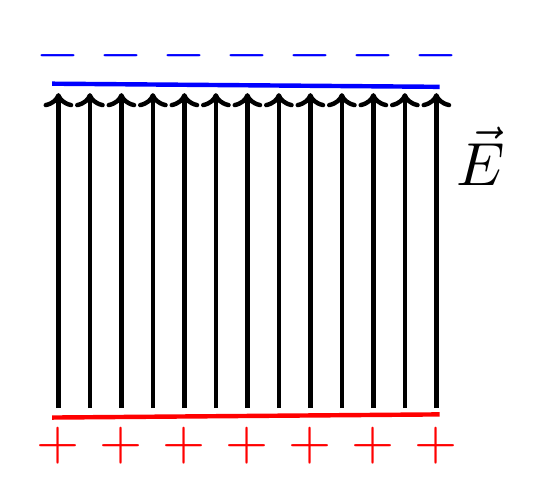
\begin{tikzpicture}[xscale=0.4,yscale=0.4]
    \draw[black, ultra thick, ->] (-6.2,-5) -- (-6.2,5);
    \draw[black, ultra thick, ->] (-5.2,-5) -- (-5.2,5);
    \draw[black, ultra thick, ->] (-4.2,-5) -- (-4.2,5);
    \draw[black, ultra thick, ->] (-3.2,-5) -- (-3.2,5);
    \draw[black, ultra thick, ->] (-2.2,-5) -- (-2.2,5);
    \draw[black, ultra thick, ->] (-1.2,-5) -- (-1.2,5);
    \draw[black, ultra thick, ->] (-0.2,-5) -- (-0.2,5);
    \draw[black, ultra thick, ->] (0.8,-5) -- (0.8,5);
    \draw[black, ultra thick, ->] (1.8,-5) -- (1.8,5);
    \draw[black, ultra thick, ->] (2.8,-5) -- (2.8,5);
    \draw[black, ultra thick, ->] (3.8,-5) -- (3.8,5);
    \draw[black, ultra thick, ->] (4.8,-5) -- (4.8,5);
    \draw[black, ultra thick, ->] (5.8,-5) -- (5.8,5);
    \node[black] at (7.2,3) {$\Scale[2.2]{\vec{E}}$};
    \draw[red, ultra thick] (-6.4,-5.3) -- (5.9,-5.2);
    \draw[blue, ultra thick] (-6.4,5.3) -- (5.9,5.2);
    \node[blue] at (-6.2,6.2) {$\Scale[2]{-}$};
    \node[blue] at (-4.2,6.2) {$\Scale[2]{-}$};
    \node[blue] at (-2.2,6.2) {$\Scale[2]{-}$};
    \node[blue] at (-0.2,6.2) {$\Scale[2]{-}$};
    \node[blue] at (1.8,6.2) {$\Scale[2]{-}$};
    \node[blue] at (3.8,6.2) {$\Scale[2]{-}$};
    \node[blue] at (5.8,6.2) {$\Scale[2]{-}$};
    \node[red] at (-6.2,-6.2) {$\Scale[2]{+}$};
    \node[red] at (-4.2,-6.2) {$\Scale[2]{+}$};
    \node[red] at (-2.2,-6.2) {$\Scale[2]{+}$};
    \node[red] at (-0.2,-6.2) {$\Scale[2]{+}$};
    \node[red] at (1.8,-6.2) {$\Scale[2]{+}$};
    \node[red] at (3.8,-6.2) {$\Scale[2]{+}$};
    \node[red] at (5.8,-6.2) {$\Scale[2]{+}$};
\end{tikzpicture}
\end{figure}

\end{frame}

\begin{frame}{Dielectrics}

Inserting a dielectric causes the negative ends of the dielectric molecules to line up with the positive plate of the capacitor and the positive ends of the dielectric molecules to line up with the negative plate of the capacitor. That is, the dielectric sets up its own electric field that weakens the electric field inside the capacitor.

\vspace{-2em}

\begin{figure}[H]
\captionsetup{width=0.8\textwidth,labelfont={color=black,bf},textfont={color=black}}
\centering
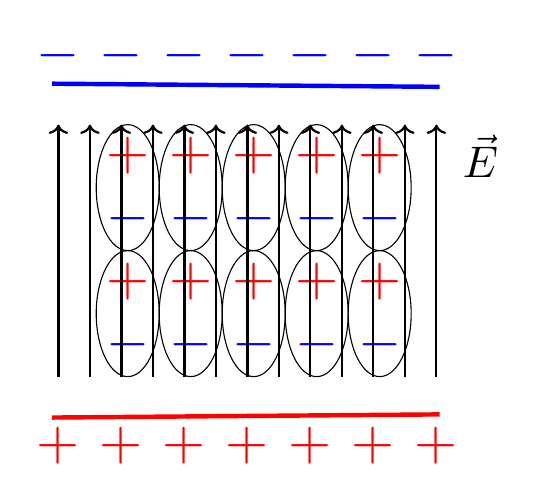
\begin{tikzpicture}[xscale=0.4,yscale=0.4]
    \draw[black] (-4,-2) ellipse (1 and 2);
    \node[blue] at (-4,-3) {$\Scale[2]{-}$};
    \node[red] at (-4,-1) {$\Scale[2]{+}$};
    \draw[black] (-4,2) ellipse (1 and 2);
    \node[blue] at (-4,1) {$\Scale[2]{-}$};
    \node[red] at (-4,3) {$\Scale[2]{+}$};
    \draw[black] (-2,-2) ellipse (1 and 2);
    \node[blue] at (-2,-3) {$\Scale[2]{-}$};
    \node[red] at (-2,-1) {$\Scale[2]{+}$};
    \draw[black] (-2,2) ellipse (1 and 2);
    \node[blue] at (-2,1) {$\Scale[2]{-}$};
    \node[red] at (-2,3) {$\Scale[2]{+}$};
    \draw[black] (0,-2) ellipse (1 and 2);
    \node[blue] at (0,-3) {$\Scale[2]{-}$};
    \node[red] at (0,-1) {$\Scale[2]{+}$};
    \draw[black] (0,2) ellipse (1 and 2);
    \node[blue] at (0,1) {$\Scale[2]{-}$};
    \node[red] at (0,3) {$\Scale[2]{+}$};
    \draw[black] (2,-2) ellipse (1 and 2);
    \node[blue] at (2,-3) {$\Scale[2]{-}$};
    \node[red] at (2,-1) {$\Scale[2]{+}$};
    \draw[black] (2,2) ellipse (1 and 2);
    \node[blue] at (2,1) {$\Scale[2]{-}$};
    \node[red] at (2,3) {$\Scale[2]{+}$};
    \draw[black] (4,-2) ellipse (1 and 2);
    \node[blue] at (4,-3) {$\Scale[2]{-}$};
    \node[red] at (4,-1) {$\Scale[2]{+}$};
    \draw[black] (4,2) ellipse (1 and 2);
    \node[blue] at (4,1) {$\Scale[2]{-}$};
    \node[red] at (4,3) {$\Scale[2]{+}$};
    \draw[black, thick, ->] (-6.2,-4) -- (-6.2,4);
    \draw[black, thick, ->] (-5.2,-4) -- (-5.2,4);
    \draw[black, thick, ->] (-4.2,-4) -- (-4.2,4);
    \draw[black, thick, ->] (-3.2,-4) -- (-3.2,4);
    \draw[black, thick, ->] (-2.2,-4) -- (-2.2,4);
    \draw[black, thick, ->] (-1.2,-4) -- (-1.2,4);
    \draw[black, thick, ->] (-0.2,-4) -- (-0.2,4);
    \draw[black, thick, ->] (0.8,-4) -- (0.8,4);
    \draw[black, thick, ->] (1.8,-4) -- (1.8,4);
    \draw[black, thick, ->] (2.8,-4) -- (2.8,4);
    \draw[black, thick, ->] (3.8,-4) -- (3.8,4);
    \draw[black, thick, ->] (4.8,-4) -- (4.8,4);
    \draw[black, thick, ->] (5.8,-4) -- (5.8,4);
    \node[black] at (7.2,3) {$\Scale[1.6]{\vec{E}}$};
    \draw[red, ultra thick] (-6.4,-5.3) -- (5.9,-5.2);
    \draw[blue, ultra thick] (-6.4,5.3) -- (5.9,5.2);
    \node[blue] at (-6.2,6.2) {$\Scale[2]{-}$};
    \node[blue] at (-4.2,6.2) {$\Scale[2]{-}$};
    \node[blue] at (-2.2,6.2) {$\Scale[2]{-}$};
    \node[blue] at (-0.2,6.2) {$\Scale[2]{-}$};
    \node[blue] at (1.8,6.2) {$\Scale[2]{-}$};
    \node[blue] at (3.8,6.2) {$\Scale[2]{-}$};
    \node[blue] at (5.8,6.2) {$\Scale[2]{-}$};
    \node[red] at (-6.2,-6.2) {$\Scale[2]{+}$};
    \node[red] at (-4.2,-6.2) {$\Scale[2]{+}$};
    \node[red] at (-2.2,-6.2) {$\Scale[2]{+}$};
    \node[red] at (-0.2,-6.2) {$\Scale[2]{+}$};
    \node[red] at (1.8,-6.2) {$\Scale[2]{+}$};
    \node[red] at (3.8,-6.2) {$\Scale[2]{+}$};
    \node[red] at (5.8,-6.2) {$\Scale[2]{+}$};
\end{tikzpicture}
\end{figure}

\end{frame}

\begin{frame}{Dielectrics}

So the dielectric sets up its own electric field that acts in opposition to the electric field of the capacitor. But recall that the voltage difference between the two plates separated a distance $d$ is
\begin{equation*}
    \left| \Delta V \right| = \int \vec{E} \cdot d\vec{\ell} = E \cdot d 
\end{equation*}

So if the electric field gets weaker, the voltage difference between the capacitor plates gets correspondingly weaker. Now recall the definition of capacitance:
\begin{equation*}
    C = \frac{Q}{\Delta V}
\end{equation*}

Charge $Q$ is fixed and $\Delta V$ decreases. So the capacitance increases!

\end{frame}

\begin{frame}{Gauss's Law in Dielectrics}

With dielectrics, we make one substitution to Gauss's law: $\epsilon_o \to \epsilon = \kappa \epsilon_o$. So Gauss's law becomes
\begin{equation*}
    \oint \vec{E} \cdot d\vec{A} = \frac{Q_{\text{enc}}}{\epsilon_o} \quad \to \quad \oint \vec{E} \cdot d\vec{A} = \frac{Q_{\text{enc}}}{\epsilon}
\end{equation*}

\end{frame}

\begin{frame}{Worked Example --- Finding the Capacitance of Concentric Spheres}

$\blacktriangleright$ Consider a spherical shell of radius $a$, nested within a larger spherical shell of radius $b$. The space between them is filled with a dielectric with dielectric constant $\kappa$.

\begin{figure}
\centering
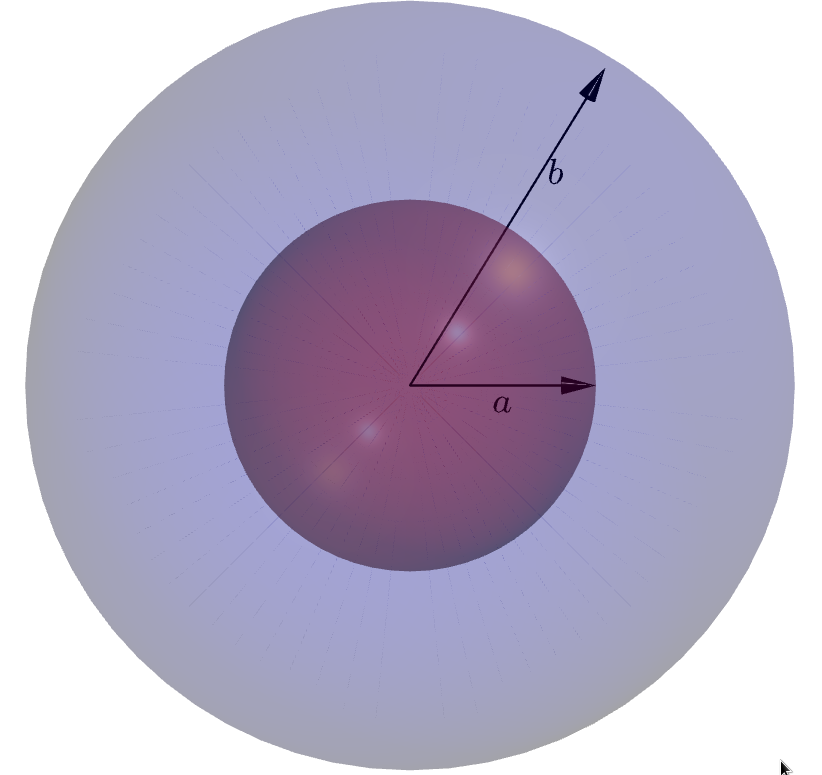
\includegraphics[height=0.5\textheight]{figures/two.png}
\end{figure}

Find the capacitance of this arrangement.

\end{frame}

\begin{frame}{Worked Example --- Finding the Capacitance of Concentric Spheres}

\textit{Solution.} Let's start with the definition of capacitance:
\begin{equation*}
    C = \frac{Q}{\Delta V}
\end{equation*}

And assume a charge of $+Q$ on the inner electrode and $-Q$ on the outer electrode:

\begin{figure}
\centering
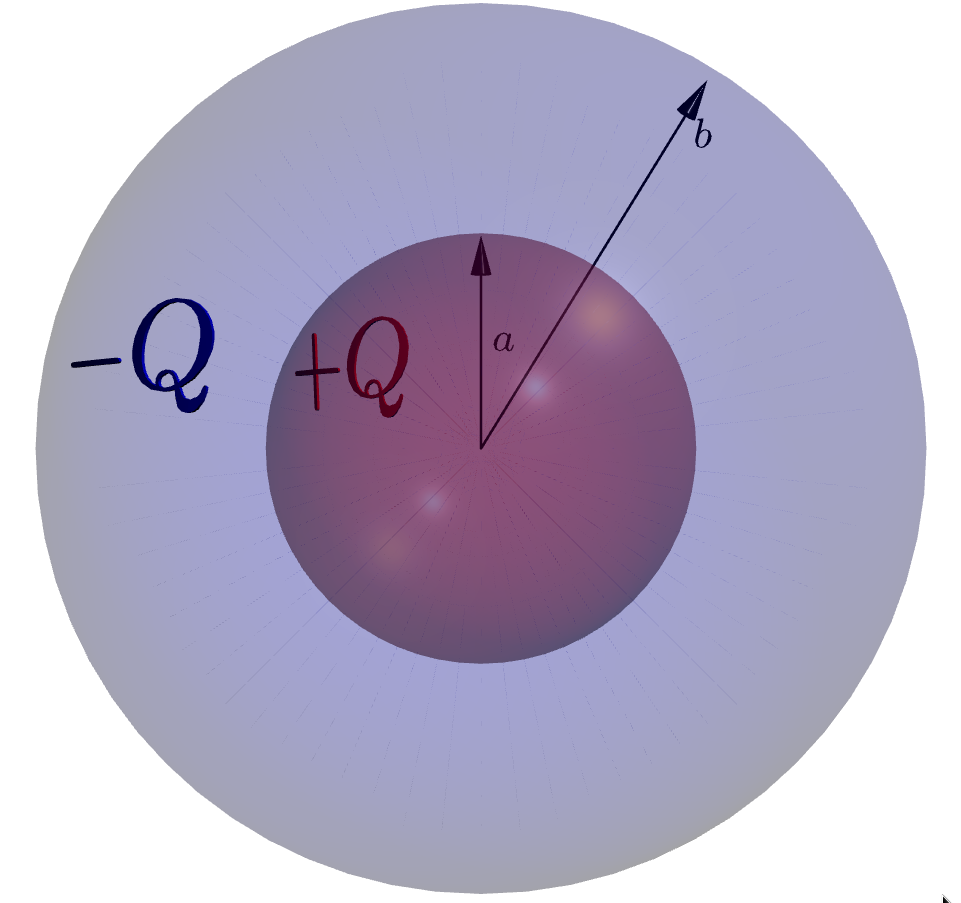
\includegraphics[height=0.36\textheight]{figures/twol.png}
\end{figure}

Now we just need to find the potential difference $\Delta V$ between the two electrodes. And for that, we need to integrate over the electric field!

\end{frame}

\begin{frame}{Worked Example --- Finding the Capacitance of Concentric Spheres}

To find the electric field, we can apply Gauss's law, which reads
\begin{equation*}
    \oint \vec{E} \cdot d\vec{A} = \frac{Q_{\text{enc}}}{\epsilon}
\end{equation*}

We want to find the electric field in between the electrodes (for $r$ such that $a < r < b$).

\end{frame}

\begin{frame}{Worked Example --- Finding the Capacitance of Concentric Spheres}

Consider a spherical Gaussian surface of radius $r$, such that $a < r < b$:

\begin{figure}
\centering
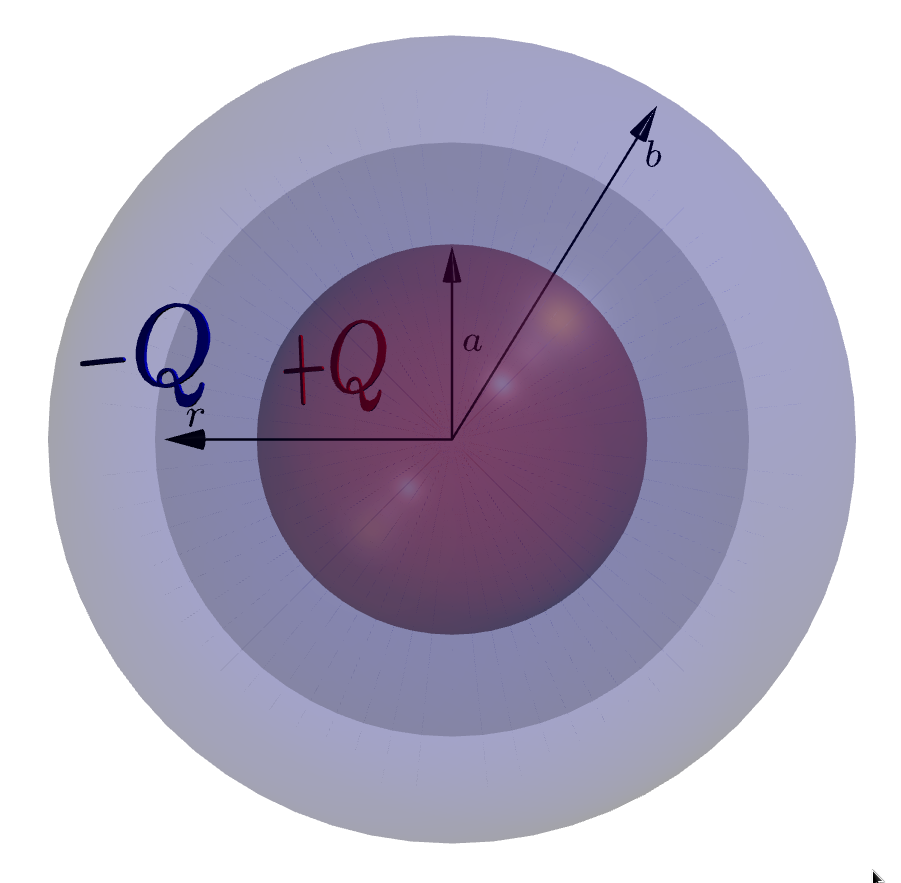
\includegraphics[height=0.36\textheight]{figures/tree.png}
\end{figure}

This Gaussian surface encloses the charge $+Q$. Moreover, its surface area is $4\pi r^2$. All pertinent symmetry arguments hold. So solving for the electric field gives
\begin{gather*}
    \oint \vec{E} \cdot d\vec{A} = \frac{Q_{\text{enc}}}{\epsilon} \implies E \left( 4\pi r^2 \right) = \frac{+Q}{\kappa \epsilon_o} \implies E = \frac{Q}{4\pi \kappa \epsilon_o r^2}
\end{gather*}

\end{frame}

\begin{frame}{Worked Example --- Finding the Capacitance of Concentric Spheres}

We can integrate this electric field to find the magnitude of the potential difference $\Delta V$ between the electrodes:
\begin{align*}
    \big| \Delta V \big| &= \int \vec{E} \cdot d\vec{\ell} \\
    &= \int_a^b \left( \frac{Q}{4\pi \kappa \epsilon_o r^2} \right)\ dr \\
    &= \frac{Q}{4\pi\kappa\epsilon_o} \int_a^b \frac{dr}{r^2} \\
    &= \frac{Q}{4\pi\kappa\epsilon_o} \left( -\frac{1}{r} \right) \bigg|_{a}^{b} \\
    &= \frac{Q}{4\pi\kappa\epsilon_o} \left( \frac{1}{a} - \frac{1}{b} \right)
\end{align*}

\end{frame}

\begin{frame}{Worked Example --- Finding the Capacitance of Concentric Spheres}

Again, the definition of capacitance is
\begin{equation*}
    C = \frac{Q}{\Delta V}
\end{equation*}

Substituting for the voltage difference $\Delta V$, we have
\begin{equation*}
    C = \frac{\cancel{Q}}{\frac{\cancel{Q}}{4\pi\kappa\epsilon_o} \left( \frac{1}{a} - \frac{1}{b} \right)} = \boxed{\frac{4\pi\kappa\epsilon_o}{\left( \frac{1}{a} - \frac{1}{b} \right)}} \blacktriangleleft
\end{equation*}

\end{frame}

\begin{frame}{Charging RC Circuits}

A \emph{charging} RC circuit might look like this:

\begin{figure}[H]
\centering
\begin{circuitikz}
    \draw (0,0) to[american voltage source,l^=$\mathscr{E}$] (0,3);
    \draw (0,3) to[nos] (4,3);
    \draw (4,3) to[resistor,l^=$R$] (4,0);
    \draw (4,0) to[capacitor,l^=$C$] (0,0);
    % \draw (0,0.9) to[resistor,l^=$R_1$,i>=$\textcolor{BLUE}{I_1}$] (0,3);
    % \draw (0,3) to[battery,invert,l^=$V_2$] (0,4);
    % \draw (3,0) to[resistor,l^=$R_2$,i>=$\textcolor{BLUE}{I_2}$] (3,4);
    % \draw (6,0) to[battery,invert,l^=$V_3$,i>=$\textcolor{BLUE}{I_3}$] (6,2.4);
\end{circuitikz}
\end{figure}

The capacitor starts out initially uncharged. At $t=0$, the switch is closed and the capacitor charges according to
\begin{equation*}
    Q(t) = Q_{\text{final}} \left( 1 - e^{-t/RC} \right)
\end{equation*}

\end{frame}

\begin{frame}{Charging RC Circuits --- A Mini Derivation}

The figure below shows an RC circuit at some time $t > 0$. The emf source $\mathscr{E}$ is charging the capacitor $C$ through the resistor $R$. A current $I$ flows through the resistor as charge $Q$ builds up on the capacitor:

\vspace{-1em}

\begin{figure}[H]
\centering
\begin{circuitikz}[scale=0.8]
    \draw (0,0) to[american voltage source,l^=$\mathscr{E}$] (0,3);
    % \draw (0,3) to[switch] (4,3);
    % \draw (1,3) to[short,*-*,i>=$I$] (1,3) node[label={[font=\small]below:$\textcolor{RED}{\text{Bottom Junction}}$}] {} to (3,3);
    \draw (0,3) to (1.5,3);
    \draw (1.5,3) to[short,*-*,i>=$I$] (2.5,3); 
    \draw (2.5,3) to (4,3);
    \draw (4,3) to[resistor,l^=$R$] (4,0);
    \draw (4,0) to[capacitor,l^=$C$] (0,0);
    % \draw (0,0.9) to[resistor,l^=$R_1$,i>=$\textcolor{BLUE}{I_1}$] (0,3);
    % \draw (0,3) to[battery,invert,l^=$V_2$] (0,4);
    % \draw (3,0) to[resistor,l^=$R_2$,i>=$\textcolor{BLUE}{I_2}$] (3,4);
    % \draw (6,0) to[battery,invert,l^=$V_3$,i>=$\textcolor{BLUE}{I_3}$] (6,2.4);
\end{circuitikz}
\end{figure}

\vspace{-1em}

If we apply Kirchhoff's Voltage Law to the circuit above, then conservation of energy requires
\begin{equation*}
    \underbrace{\hspace{1em}\mathscr{E}\hspace{1em}}_{\Delta V_{\text{emf}}} + \underbrace{\hspace{1em}-I(t) R\hspace{1em}}_{\Delta V_R} + \underbrace{\hspace{1em} -\frac{Q(t)}{C} \hspace{1em}}_{\Delta V_C} = 0
\end{equation*}

\end{frame}

\begin{frame}{Charging RC Circuits --- A Mini Derivation}

So Kirchhoff's Voltage Law gave us
\begin{gather*}
    \mathscr{E} - I(t) R - \frac{Q(t)}{C} = 0 \quad \implies \quad I(t) R + \frac{Q(t)}{C} = \mathscr{E}
\end{gather*}

The capacitor is charging, so $I = +\frac{dQ}{dt}$, which means we can express the above equation as an ordinary differential equation for the charge $Q(t)$ on the capacitor:
\begin{equation*}
    \frac{dQ(t)}{dt} + \frac{Q(t)}{RC} = \frac{\mathscr{E}}{R}
\end{equation*}

Solving this differential equation gives
\begin{equation*}
    \boxed{Q(t) = C \mathscr{E} \left( 1 - e^{-t/RC} \right) = Q_{\text{final}} \left( 1 - e^{-t/RC}\right)}
\end{equation*}

This is the same equation that's on the equation sheet and it's all we need!

\end{frame}

\begin{frame}{Charging RC Circuits}

So the charge on the capacitor is
\begin{equation*}
    Q(t) = C \mathscr{E} \left( 1 - e^{-t/RC} \right)
\end{equation*}

What if we want the current in the circuit? Current is just the time-derivative of charge:
\begin{equation*}
    I(t) = +\frac{dQ(t)}{dt} = \frac{\mathscr{E}}{R} e^{-t/RC} = I_{\text{init}} e^{-t/RC}
\end{equation*}

What if we want the potential difference across the resistor $\Delta V_R$? That just comes from Ohm's law:
\begin{equation*}
    \Delta V_R (t) = I(t) R = \mathscr{E} e^{-t/RC}
\end{equation*}

What if we want the potential difference across the capacitor $\Delta V_C$? That just comes from the definition of capacitance:
\begin{equation*}
    \Delta V_C (t) = \frac{Q(t)}{C} = \mathscr{E} \left( 1 - e^{-t/RC} \right)
\end{equation*}

\end{frame}

\begin{frame}{Discharging RC Circuits}

A \emph{discharging} RC circuit might look like this:

\begin{figure}[H]
\centering
\begin{circuitikz}
    \draw (0,0) to[capacitor,l^=$C$] (0,3);
    \draw (0,3) to[nos] (4,3);
    \draw (4,3) to[resistor,l^=$R$] (4,0);
    \draw (4,0) to (0,0);
    % \draw (0,0.9) to[resistor,l^=$R_1$,i>=$\textcolor{BLUE}{I_1}$] (0,3);
    % \draw (0,3) to[battery,invert,l^=$V_2$] (0,4);
    % \draw (3,0) to[resistor,l^=$R_2$,i>=$\textcolor{BLUE}{I_2}$] (3,4);
    % \draw (6,0) to[battery,invert,l^=$V_3$,i>=$\textcolor{BLUE}{I_3}$] (6,2.4);
\end{circuitikz}
\end{figure}

The capacitor starts out initially charged. At $t=0$, the switch is closed and the capacitor discharges according to
\begin{equation*}
    Q(t) = Q_{\text{initial}} e^{-t/RC}
\end{equation*}

\end{frame}

\begin{frame}{Discharging RC Circuits --- A Mini Derivation}

The figure below shows an RC circuit at some time $t > 0$. A capacitor $C$ is discharging itself through the resistor $R$. A current $I(t)$ flows through the resistor as charge $Q(t)$ leaves the capacitor:

\vspace{-1em}

\begin{figure}[H]
\centering
\begin{circuitikz}[scale=0.8]
    \draw (0,0) to[capacitor,l^=$C$] (0,3);
    % \draw (0,3) to[nos] (4,3);
    \draw (4,3) to[resistor,l^=$R$] (4,0);
    \draw (4,0) to (0,0);
    % \draw (0,3) to[switch] (4,3);
    % \draw (1,3) to[short,*-*,i>=$I$] (1,3) node[label={[font=\small]below:$\textcolor{RED}{\text{Bottom Junction}}$}] {} to (3,3);
    \draw (0,3) to (1.5,3);
    \draw (1.5,3) to[short,*-*,i>=$I$] (2.5,3); 
    \draw (2.5,3) to (4,3);
\end{circuitikz}
\end{figure}

\vspace{-1em}

If we apply Kirchhoff's Voltage Law to the circuit above, then conservation of energy requires
\begin{equation*}
    \underbrace{\hspace{1em} \frac{Q(t)}{C} \hspace{1em}}_{\Delta V_C} + \underbrace{\hspace{1em}-I(t) R\hspace{1em}}_{\Delta V_R} = 0
\end{equation*}

\end{frame}

\begin{frame}{Discharging RC Circuits --- A Mini Derivation}

So Kirchhoff's Voltage Law gave us
\begin{equation*}
    \frac{Q(t)}{C} - I(t) R = 0 \quad \implies \quad -I(t) R + \frac{Q(t)}{C} = 0
\end{equation*}

The capacitor is discharging, so $I=-\frac{dQ}{dt}$, which means we can express the above equation as an ordinary differential equation for the charge $Q(t)$ on the capacitor:
\begin{equation*}
    \frac{dQ(t)}{dt} + \frac{Q(t)}{RC} = 0 
\end{equation*}

Solving this differential equation gives
\begin{equation*}
    \boxed{Q(t) = Q_{\text{initial}} e^{-t/RC}}
\end{equation*}

This is the same equation that's on the equation sheet and it's all we need!

\end{frame}

\begin{frame}{Discharging RC Circuits}

So the charge on the capacitor is
\begin{equation*}
    Q(t) = Q_{\text{initial}} e^{-t/RC}
\end{equation*}

What if we want the current in the circuit? Current is just the time derivative of charge (negative here because capacitor is losing charge):
\begin{equation*}
    I(t) = -\frac{dQ(t)}{dt} = \frac{Q_{\text{init}}}{RC} e^{-t/RC} = I_{\text{init}} e^{-t/RC}
\end{equation*}

What if we want the potential difference across the resistor $\Delta V_R$? That just comes from Ohm's law:
\begin{equation*}
    \Delta V_R (t) = I(t) R = \frac{Q_{\text{init}}}{C} e^{-t/RC}
\end{equation*}

What if we want the potential difference across the capacitor $\Delta V_C$? That just comes from the defintion of capacitance:
\begin{equation*}
    \Delta V_C (t) = \frac{Q(t)}{C} = \frac{Q_{\text{init}}}{C} e^{-t/RC}
\end{equation*}

\end{frame}

\begin{frame}{AC Circuits}

An AC signal varies with time, such as that shown below:

\begin{figure}[H]
\centering
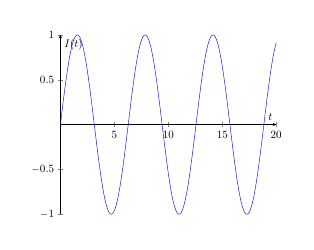
\begin{tikzpicture}[scale=0.4]
\begin{axis}[axis lines = center, xlabel = $t$, ylabel = {$I(t)$}]
\addplot[domain=0:20, samples=200, color=blue] {sin(deg(x))};
\end{axis}
\end{tikzpicture}
\end{figure}

\begin{center}
(In practice, the signal need not be sinusoidal, but that's what we'll be dealing with.)
\end{center}

We need two parameters to describe an AC signal: the amplitude (either $V_o$ or $I_o$) and the frequency $f$ (measured in \textbf{hertz} (Hz): $\SI{1}{\hertz} = \SI{1}{\text{cycle}\per\second}$). Note that the angular frequency $\omega$ and the frequency $f$ are related via
\begin{equation*}
    \omega = 2\pi f
\end{equation*}

\end{frame}

\begin{frame}{Root-Mean-Square Values}

Suppose a current is given as $I(t) = I_{\text{max}} \cos{(\omega t)}$. Its root-mean square value is
\begin{align*}
    I_{\text{rms}} &= \sqrt{\left( I^2 \right)_{\text{mean}}} = \sqrt{\left( I_{\text{max}}^2 \cos^2{\left(\omega t\right)}\right)_{\text{mean}}} = \sqrt{\frac{I_{\text{max}}^2}{2}} = \frac{I_{\text{max}}}{\sqrt{2}}
\end{align*}

In general, for a quantity that varies with time as a sinusoidal function, the rms value is the maximum value divided by $\sqrt{2}$.

The expressions for resistor circuits are pretty much still the same:
\begin{gather*}
    P = I \left( \Delta V \right) \quad \implies \quad P_{\text{mean}} = I_{\text{rms}} \left( \Delta V_{\text{rms}} \right) \\
    P = I^2 R \quad \implies \quad P_{\text{mean}} = I_{\text{rms}}^2 R \\
    \Delta V = I R \quad \implies \quad \Delta V_{\text{rms}} = I_{\text{rms}} R
\end{gather*}

\end{frame}

\begin{frame}{Resistors in AC Circuits}

Consider the circuit shown, with input signal $V(t) = V_o \cos{(\omega t)}$

\begin{figure}[H]
\centering
\begin{circuitikz}
    \draw (0,0) to[vsourcesin,l^=$V(t)$] (0,2);
    \draw (0,2) to (3,2);
    \draw (3,2) to[resistor,l^=$R$] (3,0);
    \draw (3,0) to (0,0);
\end{circuitikz}
\end{figure}

Ohm's law still holds, and the current in the circuit is
\begin{equation*}
    I(t) = \frac{V(t)}{R} = \frac{V_o}{R} \cos{(\omega t)} = I_o \cos{(\omega t)}
\end{equation*}

\end{frame}

\begin{frame}{Capacitors in AC Circuits}

Consider the circuit shown, with input signal $V(t) = V_o \cos{(\omega t)}$

\begin{figure}[H]
\centering
\begin{circuitikz}
    \draw (0,0) to[vsourcesin,l^=$V(t)$] (0,2);
    \draw (0,2) to (3,2);
    \draw (3,2) to[C,l^=$C$] (3,0);
    \draw (3,0) to (0,0);
    % \draw (0,0.9) to[resistor,l^=$R_1$,i>=$\textcolor{BLUE}{I_1}$] (0,3);
    % \draw (0,3) to[battery,invert,l^=$V_2$] (0,4);
    % \draw (3,0) to[resistor,l^=$R_2$,i>=$\textcolor{BLUE}{I_2}$] (3,4);
    % \draw (6,0) to[battery,invert,l^=$V_3$,i>=$\textcolor{BLUE}{I_3}$] (6,2.4);
\end{circuitikz}
\end{figure}

Note that the charge on the capacitor is
\begin{equation*}
    Q = C V = C \left( V_o \cos{(\omega t)} \right)
\end{equation*}

Then the current in the circuit is
\begin{equation*}
    I(t) = \frac{d}{dt} \overbrace{\left( C V_o \cos{(\omega t)} \right)}^{Q(t)} = -\underbrace{V_o \omega C}_{I_o} \sin{(\omega t)} = -I_o \sin{\left( \omega t \right)}
\end{equation*}

Note that the current goes like $\sin{(\omega t)}$ and the voltage goes like $\cos{(\omega t)}$ --- these are \emph{out of phase}!

\end{frame}

\begin{frame}{Capacitors in AC Circuits}

Observe that $I_o = V_o \omega C$. So let's define a quantity $X$ such that 
\begin{equation*}
    V_o = X I_o
\end{equation*}

This sort of resembles Ohm's Law! And in fact, $X$ is known as \emph{reactance} and it plays the role of resistance for a capacitor:
\begin{equation*}
    X = \frac{1}{\omega C}
\end{equation*}

Reactance is small for large $\omega$ and large for small $\omega$. This is a way of quantifying the statement ``with low-frequency (DC-like) input, capacitors prevent charge flow.''

\end{frame}

\begin{frame}{Resistors and Capacitors Together in AC Circuits}

Now consider the following circuit:

\begin{figure}[H]
\centering
\begin{circuitikz}
    \draw (0,0) to[vsourcesin,l^=$V(t)$] (0,3);
    \draw (0,3) to (3,3);
    \draw (3,3) to[R,l^=$R$] (3,1.2);
    \draw (3,1.2) to[C,l^=$C$] (3,0);
    \draw (3,0) to (0,0);
\end{circuitikz}
\end{figure}

Now we'll define the \emph{impedance}, $Z$, as follows:
\begin{equation*}
    Z = \sqrt{R^2 + X^2} = \sqrt{R^2 + \frac{1}{\left( \omega C \right)^2}}
\end{equation*}

The impedance is the total effective resistance (we can't simply add $X$ and $R$). The rms current through the circuit comes from
\begin{equation*}
    V_{\text{rms}} = I_{\text{rms}} Z
\end{equation*}

where $V_{\text{rms}}$ is the input signal.

\end{frame}

\begin{frame}{Low-Pass Filters}

The output voltage is measured across the capacitor on a low-pass filter:

\begin{figure}[H]
\centering
\begin{circuitikz}
    \draw (0,0) to[vsourcesin,l^=$V_{\text{in}}$] (0,3);
    \draw (0,3) to[R,l^=$R$] (3,3);
    \draw (3,3) to[C,l_=$C$,v^<=$V_{\text{out}}$] (3,0);
    \draw (3,0) to (0,0);
\end{circuitikz}
\end{figure}

The gain is the ratio of the output voltage to the input voltage:
\begin{gather*}
    \text{Gain} = \frac{V_{\text{out, rms}}}{V_{\text{in, rms}}} = \frac{V_{C, \text{ rms}}}{V_{\text{in, rms}}} = \frac{I_{\text{rms}}\ X_C}{I_{\text{rms}}\ Z} = \frac{X_C}{Z} \\
    \implies \text{Gain} = \frac{\left( \frac{1}{\omega C} \right)}{\sqrt{R^2 + \left( \frac{1}{\omega C} \right)^2}} = \frac{1}{\sqrt{\left( \omega R C \right)^2 + 1}}
\end{gather*}

\end{frame}

\begin{frame}{High-Pass Filters}

The output voltage is measured across the resistor on a high-pass filter:

\vspace{-0.8em}

\begin{figure}[H]
\centering
\begin{circuitikz}
    \draw (0,0) to[vsourcesin,l^=$V_{\text{in}}$] (0,3);
    \draw (0,3) to[C,l^=$C$] (3,3);
    \draw (3,3) to[R,l_=$R$,v^<=$V_{\text{out}}$] (3,0);
    \draw (3,0) to (0,0);
\end{circuitikz}
\end{figure}

The gain is the ratio of the output voltage to the input voltage:
\begin{gather*}
    \text{Gain} = \frac{V_{\text{out, rms}}}{V_{\text{in, rms}}} = \frac{V_{R, \text{ rms}}}{V_{\text{in, rms}}} = \frac{I_{\text{rms}}\ R}{I_{\text{rms}}\ Z} = \frac{R}{Z} \\
    \implies \text{Gain} = \frac{R}{\sqrt{R^2 + \left( \frac{1}{\omega C} \right)^2}} = \frac{\omega R C}{\sqrt{\left( \omega R C \right)^2 + 1}}
\end{gather*}

\end{frame}

\end{document}
